%%%%%%%%%%%%%%%%%%%%%%%%%%%%%%%%%%%%%%%%% 
\documentclass[mathpazo]{aamm}
%%%%% journal  info %%%%%%%%%
\setcounter{page}{1}
\renewcommand\thisnumber{x}
\renewcommand\thisyear {2016}
\renewcommand\thismonth{xxx}
\renewcommand\thisvolume{xx}
%%%%%%%%   end  %%%%%%%%%%%%%

%%%%% author macros %%%%%%%%%
% place your own macros HERE
%%%%% end %%%%%%%%%

\usepackage{graphicx} % Required for the inclusion of images
\usepackage{epstopdf} % eps to pdf
\usepackage{epsfig}
\usepackage{amsmath} % Required for some math elements 
\usepackage[colorlinks, linkcolor=black, anchorcolor=blue,
citecolor=black]{hyperref}
\usepackage{algorithm}
\usepackage{enumerate}
\usepackage{algpseudocode}
\usepackage{tikz}
\usepackage{pgflibraryarrows}
\usepackage{pgflibrarysnakes}
\usepackage{subfig}
\usepackage{booktabs} 

\usepackage{multirow}
% ----------------------------------------------------------------------------------------
%	DOCUMENT INFORMATION
% ----------------------------------------------------------------------------------------
\begin{document}

%%%%% title and author(s):
% \markboth{Author(s)}{Short Title}
% \title{Title}

\markboth{Yirong Wu and Heyu Wang}{Moving mesh FEM for unsteady NS flow}
\title{Moving mesh finite element method for unsteady Navier-Stokes flow}

% single author:
% \author[AUTHOR]{AUTHOR\corrauth}
% \address{address of AUTHOR}
% \email{{\tt email address of AUTHOR} (AUTHOR)}
%\author[Only Author]{Only Author\corrauth}
%\address{School of Mathematical Sciences, Beijing International University,
%Beijing 12345, China.}
%\email{{\tt email@address} (Only Author)}

% multiple authors:
% Please mark \corrauth after the name of the corresponding author.
% different addresses:
%\author[AUTHOR1 and AUTHOR2]{AUTHOR1\affil{1}\comma\corrauth and AUTHOR2\affil{2}}
%\address{\affilnum{1}\ address of AUTHOR1\\
%\affilnum{2}\ address of AUTHOR2}
%
%same address:
%\author[AUTHOR1, AUTHOR2 and AUTHOR3]{AUTHOR1, AUTHOR2\corrauth and AUTHOR3}
%\address{address of AUTHOR1, AUTHOR2 and AUTHOR3}
%
%\emails{{\tt email of AUTHOR1} (AUTHOR1), {\tt email of AUTHOR2} (AUTHOR2), {\tt email of AUTHOR3} (AUTHOR3)}
%
%same address:
\author[Yirong Wu and Heyu Wang]{Yirong Wu and Heyu Wang\corrauth}
\address{School of Mathematical Science, ZheJiang University, HangZhou,
  310027, China}

\emails{{\tt wuwuyiyirongrong@163.com} (Yirong Wu), {\tt
    wang.heyu@gmail.com} (Heyu Wang)}

%%%%% Begin Abstract %%%%%%%%%%%
\begin{abstract}
    In this paper, we use moving mesh fintie element method based upon
    $4P_1-P_1$ element to solve the time-dependent Navier-Stokes
    equations in 2D. Two-layer nested meshes are used including
    velocity mesh and pressure mesh, and velocity mesh can be obtained
    by globally refining pressure mesh. We use hierarchy
    geometry tree to store the nested meshes. This data
    structure make convienence for adaptive mesh method and the
    construction of multigrid preconditioning. 
    Seveval numerical problems are used to show the effect of moving mesh. \\
\end{abstract}
%%%%% end %%%%%%%%%%%

%%%%% Keywords %%%%%%%%%%%
\keywords{Navier-Stokes system, $4P_1-P_1$, hierarchy geometry tree,
  moving mesh method.}

%%%% maketitle %%%%%
\maketitle

%%%% Start %%%%%%
\section{Introduction}
    \label{sec1} It is important that solving incompressible
    Navier-Stokes equations by mixed finite element method. In order to
    satisfy the LBB condition, one way is to enhance velocity space
    relative to pressure, for example Taylor-Hood element. The other is imposing
    constraint on pressure space, such as stablized $P_1-P_1$,
    $P_1-P_0$(\cite{li2009performance},\cite{bochev2006stabilization}). 
    In practical computing, adaptive scheme is often used to decrease the
    computitional cost for efficency. Meanwhile, it can improve the quality
    of solutions locally see \cite{popiolek2006numerical}. There are some works
    using h-adaptive $P_2-P_1$ element because of simplicity, see
    (\cite{danaila2014newton},\cite{ebeida2009unsteady},
    \cite{berrone2009space}) for detail. However, if domain has some
    corners or solutions have some singularities, we tend to use lower
    order approximations in engineering computation. Adaptive method with
    stablized $P_1-P_1$ and $P_1-P_0$ elements are proposed in
    \cite{zheng2010posteriori}. In \cite{di2005moving},
    dual element $P_1-P_0$ is used for moving mesh method. It has some 
    technical difficulties in applying adaptive mesh based on unstable
    element pairs. So $P_1\text{iso}P_2P_1$
    (\cite{fujima1998iso},\cite{bercovier1979error},
    \cite{vanden2009kinetic}) is considered. In
    \cite{bercovier1979error}, it is pointed out that
    $P_1isoP_2P_1$  satisfies the LBB condition. Four velocity
    elements can be obtained by refining the pressure element one
    time as Figure \ref{fig::p-v} shows. Note that
    $P_1\text{iso}P_2P_1$ element is based on one set of mesh, so
    basis functions of pressure element are obtained by the
    interpolation of velocity basis functions. This will increase
    caculation.
    
    In this paper, we choose $4P_1-P_1$ finite element pair. It has the
    same structure as $P_1\text{iso}P_2P_1$ pair, so the LBB condition
    is natrually satisfied. However, The basis functions of both
    velocity and pressure elements are all standard $P_1$ element
    without any extra interpolation. We use the hierarchy
    geometry tree which was proposed in \cite{li2005multi} to store
    the mesh structure of  $4P_1-P_1$ pair.

    Moving mesh finite element methods have been developed by a lot
    of works such as
    \cite{Winslow1966NUMERICAL},\cite{dvinsky1991adaptive}, \cite{cao1999anr},
    \cite{li2001mesh}. In \cite{li2001mesh}, a moving mesh finite element
    method based upon harmonic map was proposed. The authors in \cite{di2005moving}
    extended the moving scheme to solve incompressible Navier-Stokes
    equations. However, the boundary conditions of numerical
    experiments in \cite{di2005moving} are periodic. In this paper, we
    use moving mesh method based on $4P_1-P_1$ pair and the boundary
    conditions are general Dirichlet and Neumann boundary conditions.

    \begin{figure}
      \centering    
      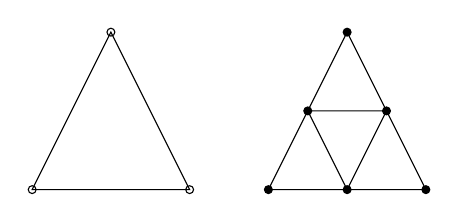
\begin{tikzpicture}
        % 三角形
        \draw (2, 1) -- (4, 1) -- (3, 3) -- cycle;
        % 三个顶点
        \draw (2, 1) circle(0.05cm);
        \draw (4, 1) circle(0.05cm);
        \draw (3, 3) circle(0.05cm);
        % 四个三角形
        \draw (5, 1) -- (6, 3) -- (7, 1) -- cycle;
        \draw (5.5, 2) -- (6.5, 2) -- (6, 1) -- cycle;
        % 六个顶点
        \draw [fill = black] (5, 1) circle(0.05cm);
        \draw [fill = black] (6, 3) circle(0.05cm);
        \draw [fill = black] (7, 1) circle(0.05cm);
        \draw [fill = black] (5.5, 2) circle(0.05cm);
        \draw [fill = black] (6.5, 2) circle(0.05cm);
        \draw [fill = black] (6, 1) circle(0.05cm);
      \end{tikzpicture}
      \caption{Left: pressure $p$ element, $\circ$ for degrees of $p$; 
               right: four velocity $v$ elements, $\bullet$ for degrees
               of $v$.}
      \label{fig::p-v}       
    \end{figure}
      
       The layout of the paper is arraged as follows. In section 2, we
    introduce the Navier-Stokes governing equations. In section 3, we
    illustrate data structure for finite element pair $4P_1-P_1$, In
    section 4, $4P_1-P_1$ pair is used to approximate the governing
    equations. Next, the AMG preconditioner for steady
    stokes equations is shown. In section 6, the moving mesh
    strategy is given. Then we present numerical experiements in section 7. 
    Finaly, we give the conclusions in this section.

% ----------------------------------------------------------------------------------------
%	SECTION 1
% ----------------------------------------------------------------------------------------
\section{Governing Equation}
    \label{sec2} Following \cite{elman2005finite}, we
    give nondimentional incompressible Navier-Stokes equations as
    follows:
    
    \begin{equation}
      \begin{array}{rcl}
         \partial_t \mathbf{u} - \frac{1}{Re} \nabla^2 \mathbf{u} +
        (\mathbf{u} \cdot \nabla )\mathbf{u} + \nabla p & =
        & \mathbf{f},\\
        \nabla \cdot \mathbf{u} & = & 0.
      \end{array}
      \label{eq::NS}
    \end{equation}

    The variable $\mathbf{u}$ is velocity and the scalar
    variable $p$ is pressure. The phisical domain is
    $\Omega$. Reynolds number $Re :=
    \frac{UL}{\nu}$, where $L$ represents a characteristic length scale
    for $\Omega$, $U$ is the mean velocity
    of the inflow and $\nu > 0$ is the constant kinematic
    viscosity. The initial boundary value problem of the system
    (\ref{eq::NS}), with initial and boundary conditions on $\partial
    \Omega = \partial \Omega_D \bigcup \partial \Omega_N$:
    \begin{equation}
      \begin{array}{ll}
        \mathbf{u} = \mathbf{w},& \mbox{on} \partial \Omega_D \times [0,
        T]\\
        \frac{1}{Re} \displaystyle \frac{\partial \mathbf{u}}{\partial n} - \mathbf{n}p =
        \mathbf{0}, & \mbox{ on } \partial \Omega_N \times [0, T],  \\
        \mathbf{u}|_{t = 0} = \mathbf{u_0}, & \mbox{in} \Omega, 
      \end{array}
      \label{eq::bc}
    \end{equation} 
    where $\mathbf{n}$ denotes the outward normal to the boundary. 

    % Let $L$ represent a characteristic length scale for the domain
    % $\Omega$. Let $U$ be the maximum value of velocity on the inflow,
    % then the Reynolds number denotes:
    % \begin{equation}
    %   Re := \frac{UL}{\nu}.
    % \end{equation}
    
% ----------------------------------------------------------------------------------------
%	SECTION 2
% ----------------------------------------------------------------------------------------
\section{Illustration of the $4P_1-P_1$ element}
\label{sec3} From \cite{bercovier1979error}, we know that
   $P_1\text{iso}P_2P_1$ element satisfies the LBB condition. This
   element pair is based on only one set of mesh for instance velocity mesh
   as shown in Figure \ref{fig::p1isop2p1}. The velocity space is represented
   by standard $P_1$ basis 
   functions, while pressure space is represented by piecewise linear on the larger 
   $P_2$ element. So the basis function on node $1$ of pressure
   element is $\tilde{N}_1 = N_1 + (N_a + N_b)/2$. This
   interpolation will make caculation complicated.  
   \begin{figure}
     \centering
     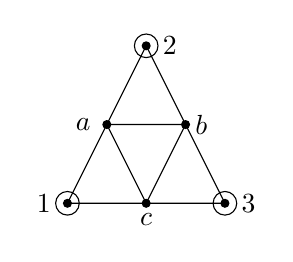
\begin{tikzpicture}
       % 四个三角形
       \draw (5, 1) -- (6, 3) -- (7, 1) -- cycle;
       \draw (5.5, 2) -- (6.5, 2) -- (6, 1) -- cycle;
       % 六个顶点, 三个压力顶点
       \draw [fill = black] (5, 1) circle(0.05cm);
       \draw (5, 1) circle(0.15cm);
       \draw [fill = black] (6, 3) circle(0.05cm);
       \draw (6, 3) circle(0.15cm);
       \draw [fill = black] (7, 1) circle(0.05cm);
       \draw (7, 1) circle(0.15cm);
       \draw [fill = black] (5.5, 2) circle(0.05cm);
       \draw [fill = black] (6.5, 2) circle(0.05cm);
       \draw [fill = black] (6, 1) circle(0.05cm);

       % 标号.
       % 三个顶点标号.
       \draw (4.7, 1) node {$1$};
       \draw (6.3, 3) node {$2$};
       \draw (7.3, 1) node {$3$};
       % 三个中点编号
       \draw (5.2, 2) node {$a$};
       \draw (6.7, 2) node {$b$};
       \draw (6, 0.8) node {$c$};
     \end{tikzpicture}
     \caption{$P_1\text{iso}P_2P_1$ pair, pressure degrees of
       freedom are only stored in vertices marked by circles.}
     \label{fig::p1isop2p1}
   \end{figure}  
   Whereas $4P_1-P_1$ element is based on two nested
   meshes including velocity and pressure mesh. So both velocity and
   pressure spaces are represented by standard $P_1$ element. This 
   will simplify matrix assembly. We use the hierarchy geometry tree in 
   \cite{li2005multi} to store the nested meshes, as Figure
   \ref{fig::hgrometrytree} shows.
 
   \begin{figure}[h]
     \subfloat[One time uniform refined mesh]{
       \begin{minipage}[t]{0.4\textwidth}
         \centering
         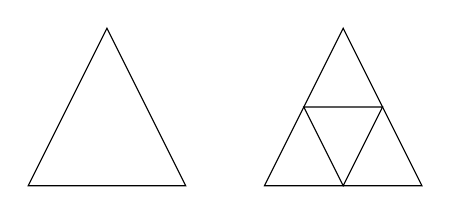
\begin{tikzpicture}
           % 三角形
           \draw (2, 1) -- (4, 1) -- (3, 3) -- cycle;
           \draw (5, 1) -- (6, 3) -- (7, 1) -- cycle;
           \draw (5.5, 2) -- (6.5, 2) -- (6, 1) -- cycle;
         \end{tikzpicture}
       \end{minipage}
     }
     \subfloat[its hierarchy tree]{
       \begin{minipage}[t]{0.6\textwidth}
         \centering
         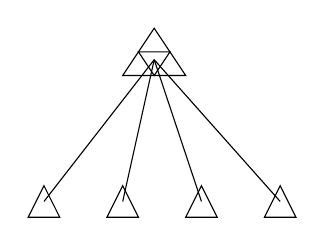
\begin{tikzpicture}
           %五个小三角形
           \draw (1.0, 0.0) -- (1.2, 0.4) -- (1.4, 0.0) -- cycle;
           \draw (2.0, 0.0) -- (2.2, 0.4) -- (2.4, 0.0) -- cycle;
           \draw (3.0, 0.0) -- (3.2, 0.4) -- (3.4, 0.0) -- cycle;
           \draw (4.0, 0.0) -- (4.2, 0.4) -- (4.4, 0.0) -- cycle;
           \draw (2.6, 2.4) -- (2.2, 1.8) -- (3.0, 1.8) -- cycle;
           \draw (2.4, 2.1) -- (2.6, 1.8) -- (2.8, 2.1) -- cycle;
           %四条线
           \draw (2.6, 2.0) -- (1.2, 0.2);
           \draw (2.6, 2.0) -- (2.2, 0.2);
           \draw (2.6, 2.0) -- (3.2, 0.2);
           \draw (2.6, 2.0) -- (4.2, 0.2);
         \end{tikzpicture}
       \end{minipage}
     }
     \caption{Hierarchy tree structure}
     \label{fig::hgrometrytree}
   \end{figure}
   Notice that two meshes are used, the $1-1$ index between them are
   needed. By traversing all pressure elements one time, we can acquire the $1-1$
   index based on the hierarchy geometry tree as Algorithm \ref{alg::index} shown.  
   \begin{algorithm}
     \caption{Make index between velocity elements and pressure elements}
     \begin{algorithmic}[1]
       \State \text{achieveiterator} $\gets$ \text{irregualerMeshV.beginActiveElement()}
       \State \text{enditerator} $\gets$ \text{irregualerMeshV.endActiveElement()}
     
       \While {\text{achieveiterator} $\neq$ \text{enditerator}}
           \State \text{int index-v-element} $\gets$
                   \text{achieveiterator}$-\rangle$ \text{index}
           \State \text{HElement} $\langle$ \text{DIM,
                   DIM}$\rangle \ast$ \text{parent} $\gets$
                   \text{activeiterator}$-\rangle$ \text{parent}
           \State \text{int index-p-element} $\gets$
                   \text {parent}$-\rangle$ \text{index}
           \State \text{int n}$\_$\text{child} $\gets$
                   \text{parent}$-\rangle$ \text{n}$\_$\text{child}
           \State
                  \text{index-p2v[index-p-element].resize}(\text{n}$\_$\text{child})
           \While {$i \geq 0$ \textbf{and} $i < $ \text{n}$\_$\text{child}}
                  \State \text{HElement}$\langle$\text{DIM,DIM}$\rangle$ $\ast$\text{chi}
                         $\gets$ \text{parent}$-\rangle$\text{child[i]}
                  \State \text{int index-v-element} $\gets$
                         \text{child}$-\rangle$\text{index}
                  \State \text{index-p2v[index-p-element][i]} $\gets$
                         \text{index-v-element}
                  \State \text{index-v2p[index-v-element]} $\gets$ \text{index-p-element}       
           \EndWhile
       \EndWhile
     \end{algorithmic}
     \label{alg::index}
   \end{algorithm}
   After the index built, we can just only use $P_1$ element to
   assemble divergence matrix for velocity and pressure.
% ----------------------------------------------------------------------------------------
%	SECTION 3
% ----------------------------------------------------------------------------------------
\section{Finite Element Approximation}
    \label{sec4} We define the solution and test spaces as
    \begin{eqnarray}
      \mathbf{H}_E^1 & := & \left\{ \mathbf{u} \in \mathcal{H}^1(\Omega)^d \big|
        \mathbf{u} = \mathbf{w} \mbox{ on } \partial \Omega_D \right\},\\
      \mathbf{H}_{E_0}^1 & := & \left\{ \mathbf{v} \in \mathcal{H}^1(\Omega)^d \big|
        \mathbf{u} = \mathbf{0} \mbox{ on } \partial \Omega_D \right\}.
    \end{eqnarray}
    Variational formulation of \eqref{eq::NS} is to find  $(\mathbf{u}, p) \in
   \mathbf{H}_E^1 \times L_2(\Omega)$ such that
   \begin{eqnarray}
     \int_{\Omega}\frac{\partial \mathbf{u}}{\partial t} \cdot \mathbf{v} + 
     \frac{1}{Re} \int_\Omega \nabla \mathbf{u} : \nabla \mathbf{v} + \int_\Omega \left(
       \mathbf{u} \cdot \nabla \mathbf{u} \right) \cdot \mathbf{v} - \int_{\Omega} p
     \left( \nabla \cdot \mathbf{v} \right) & =  &\int_\Omega \mathbf{f} \cdot
     \mathbf{v}, \\
     \int_\Omega q \left( \nabla \cdot \mathbf{u} \right) & = & 0,
     \label{eq::NS_weakform}
   \end{eqnarray}
   for $\forall (\mathbf{v}, q) \in \mathbf{H}_{E_0}^1 \times
   L_2(\Omega)$,  where $\nabla \mathbf{u} : \nabla \mathbf{v} = \nabla v_x \cdot \nabla u_x + \nabla
   v_y \cdot \nabla u_y$ in 2D.

   Assume $\mathcal{T}_H$ is a triangulation of domain $\Omega$ for
   pressure mesh with mesh parameter $H = max_{T \in \mathcal{T}_H} diam(T)$,
   $\mathcal{T}_{h}(h = 1/2H)$ is the triangulation for velocity mesh.
   Two finite element spaces $X_E^h \subset \mathcal{H}_E$ and $P^H
   \subset L_2(\Omega)$ are seperatly on $\mathcal{T}_{h}$
   and $\mathcal{T}_H$.
      
   So the discreted weak formulation of \eqref{eq::NS_weakform} is: find
   $(\mathbf{u}_h, p_H) \in X_E^h \times P^H$ such that
   \begin{equation}
     \begin{aligned}
       &\int_{\Omega}\frac{\partial \mathbf{u}_h}{\partial t} \cdot \mathbf{v}_h
       + \frac{1}{Re} \int_\Omega \nabla \mathbf{u}_h : \nabla \mathbf{v}_h  \\
       + & \int_\Omega \left( \mathbf{u}_h \cdot \nabla \mathbf{u}_h \right)
       \cdot \mathbf{v}_h - \int_\Omega p_H \left( \nabla \cdot \mathbf{v}_h
       \right) & = &\int_\Omega \mathbf{f} \cdot \mathbf{v}_h, &\quad
       \forall \mathbf{v}_h \in \mathbf{X}_0^h,  \\
       & \int_\Omega q_h \left( \nabla \cdot \mathbf{u}_h \right) & = &0,&
       \quad \forall q_h \in P^H.
       \label{eq::discreted_weak}
     \end{aligned}
   \end{equation}

   At the time discretization, we use linear backward Euler scheme,
   which linearizes the nonlinear term $\mathbf{u}_h^{n + 1}
   \cdot \nabla \mathbf{u}_h^{n + 1}$ with $\mathbf{u}_h^{n} \cdot \nabla
   \mathbf{u}_h^{n + 1}$. Let $\{\phi_j \}_{j = 1}^n$ and $\{\psi_k\}_{k = 1}^m$ be linear basis
   functions for velocity and pressure. Then $u_{h,x}, u_{h,y}, p_H$ can be written as follows:
   \begin{equation}
     u_{h,x} = \sum_{j = 1}^n \alpha_{x,j} \phi_j, \quad v_{h,x} = \sum_{j = 1}^n \alpha_{y,j}
     \phi_j, \quad p_H = \sum_{k = 1}^m \alpha_{p,k} \psi_k. 
     \label{eq::solutions_components_NS}
   \end{equation} 
   Substituting \eqref{eq::solutions_components_NS} into \eqref{eq::discreted_weak}, 
   then a linear system
   \begin{equation}
     \left[
       \begin{array}{lll}
         \frac{1}{dt} M + \frac{1}{Re} A  + W & 0 & B_x^T \\
         0 & \frac{1}{dt} M  +\frac{1}{Re} A + W & B_y^T \\
         B_x & B_y & 0
       \end{array}
     \right]
     \left[
       \begin{array}{c}
          \alpha_x \\
          \alpha_y \\
          \alpha_p
       \end{array}
     \right] = 
     \left[
       \begin{array}{c}
         f_x \\
         f_y \\
         g
       \end{array}
     \right],
     \label{eq::linear_system}
   \end{equation}
   is obtained, where $\alpha_x = (\alpha_{x,1},\cdots,\alpha_{x,n_u})^T, \alpha_y
   = (\alpha_{y,1},\cdots,\alpha_{y,n_u})^T, \alpha_p =
   (\alpha_{p,1},\cdots, \alpha_{p,n_p})^T$, $dt$ is the time step.
   Mass matrix $M$, Laplacian matrix $A$, convection-diffusion
   matrix $W$ and divergence matrix $B_x$ are defined as following: 
   \begin{eqnarray}
     \begin{aligned}
       A = [a_{ij}], && a_{ij} = \int_\Omega \nabla \phi_j \cdot \nabla
       \phi_i, \\
       M = [m_{ij}], && m_{ij} = \int_{\Omega}\phi_j \phi_i, \\
       W = [w_{ij}], && w_{ij} = \int_{\Omega}(\mathbf{u}_h^n \cdot \nabla
       \phi_j) \phi_i, \\
       B_x = [b_{ij}], && b_{ij} = \int_{\Omega}{\frac{\partial
           \phi_j}{\partial x} \psi_i}.
     \end{aligned}  
   \end{eqnarray}
   The right hand side terms $f_x, f_y, g$ seperatly are
   % \begin{eqnarray}
   %   f_x = [f_i], && f_i = \int_\Omega (\frac{u_{h,x}^{(n)}}{dt} - (u_{h,x}^{(n)}
   %     \frac{\partial u^{(n)}}{\partial x} + u_{h,y}^{(n)} \frac{\partial
   %     u_{h,x}^{(n)}}{\partial y})) \phi_i \notag \\
   %   f_y = [f_i], && f_i = \int_\Omega (\frac{u_{h,y}^{(n)}}{dt} - (u_{h,x}^{(n)}
   %     \frac{\partial u_{h,y}^{(n)}}{\partial x} + u_{h,y}^{(n)} \frac{\partial
   %       u_{h,y}^{(n)}}{\partial y})) \phi_i \notag \\
   %   g = [g_k], && g_i = 0. \notag
   % \end{eqnarray}
   \begin{eqnarray}
     \begin{aligned}
       f_x = [f_{x,i}], && f_{x,i} = \int_\Omega (\frac{u_{h, x}^{(n)}}{dt})
       \phi_i, \\
       f_y = [f_{y,i}], && f_{y,i} = \int_{\Omega}(\frac{u_{h,
           y}^{(n)}}{dt}) \phi_i,  \\
       g = [g_k], && g_k = 0.
     \end{aligned}
   \end{eqnarray}  

    \begin{figure}
      \centering    
      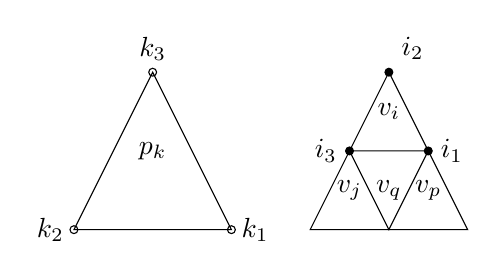
\begin{tikzpicture}
        % 三角形
        \draw (2, 1) -- (4, 1) -- (3, 3) -- cycle;
        % 三个顶点
        \draw (2, 1) circle(0.05cm);
        \draw (4, 1) circle(0.05cm);
        \draw (3, 3) circle(0.05cm);
        \draw (3, 2) node{$p_k$};
        % 三个顶点标号.
        \draw (1.7, 1) node {$k_2$};
        \draw (4.3, 1) node {$k_1$};
        \draw (3, 3.3) node {$k_3$};
        % 四个三角形
        \draw (5, 1) -- (6, 3) -- (7, 1) -- cycle;
        \draw (5.5, 2) -- (6.5, 2) -- (6, 1) -- cycle;
        % 六个顶点
        \draw [fill = black](6.5, 2) circle(0.05cm);
        \draw [fill = black](5.5, 2) circle(0.05cm);
        \draw [fill = black](6, 3) circle(0.05cm);
        % 三个顶点标号.
        \draw (6.8, 2) node {$i_1$};
        \draw (6.3, 3.3) node {$i_2$};
        \draw (5.2, 2) node {$i_3$};
        % 单元标记.
        \draw (6, 2.5) node {$v_i$};
        \draw (5.5, 1.5) node {$v_j$};
        \draw (6.5, 1.5) node {$v_p$};
        \draw (6, 1.5) node {$v_q$};
      \end{tikzpicture}
      \caption{Left: the k-th pressure element $p_k$; 
        right: four velocity elements corresponding to $p_k$.}
      \label{fig::matrix_assemble}       
    \end{figure}
   
   Here, we concentrate on the assembling of divergent matrix. Take 
   $B_x^T$ for instance. Let $\triangle_{v_i}$ be a velocity element,
   we can find the corresponding pressure element $\triangle_{p_k}$ 
   (see Figure \ref{fig::matrix_assemble}) by the index built in the last
   section. The local index of basis function is shown. $\phi_{i_1},
   \phi_{i_2}, \phi_{i_3}$ are the standard linear triangle basis
   functions defined on $\triangle_{v_i}$. While
   $\psi_{k_1}, \psi_{k_2}, \psi_{k_3}$ are defined on
   $\triangle_{p_k}$. Therefor, the element contribution matrix of $B_x^T$ is 
   \begin{equation}
     \left[
     \begin{array}{lll}
       \int_{\triangle_{v_i}}\psi_{k_1} \frac{\partial
         \phi_{i_1}}{\partial x} & \int_{\triangle_{v_i}} \psi_{k_2}
       \frac{\partial \phi_{i_1}}{\partial x} & \int_{\triangle_{v_i}}
       \psi_{k_3} \frac{\partial \phi_{i_1}}{\partial x} \\
       \int_{\triangle_{v_i}} \psi_{k_1} \frac{\partial
         \phi_{i_2}}{\partial x} & \int_{\triangle_{v_i}} \psi_{k_2}
       \frac{\partial \phi_{i_2}}{\partial x} & \int_{\triangle_{v_i}}
       \psi_{k_3} \frac{\partial \phi_{i_2}}{\partial x} \\
       \int_{\triangle_{v_i}} \psi_{k_1} \frac{\partial
         \phi_{i_3}}{\partial x} & \int_{\triangle_{v_i}} \psi_{k_2}
       \frac{\partial \phi_{i_3}}{\partial x} & \int_{\triangle_{v_i}}
       \psi_{k_3} \frac{\partial \phi_{i_3}}{\partial x}
     \end{array}
   \right]
   \label{eq::element_matrix}
   \end{equation}
   
   Add the entries of \eqref{eq::element_matrix} to correspondent positions
   $(i_1,k_1)$, $(i_1, k_2)$, $(i_1, k_3)$, $(i_2, k_1)$, $(i_2, k_2)$,
   $(i_2,k_3)$, $(i_3, k_1)$, $(i_3, k_2)$, $(i_3, k_3)$ in $B_x^T$. 
   After traversing all the velocity elements and repeat above action,
   $B_x^T$ is completely assembled. Similarly, we can assemble matrix
   $B_y^T$.

   Conversly, by the index of pressure element $p_k$, we can find the 
   corresponding four small velocity elements $v_i, v_j, v_p, v_q$ see
   Figure \ref{fig::matrix_assemble}. $B_x$ can be assembled by the
   similar process of assembling of $B_x^T$.
   % After seperatly assembling the
   % element $p_k$ with velocity elements $v_i, v_j, v_p, v_q$,  one
   % pressure element matrix is built and add it to $B_x$. Repeat above 
   % action until all the pressure elements are traversed. Therefor,
   % $B_x$ is completely built. The assembling of $B_y$ is in the same way.    
   
   If we get rid of time term and nonlinear $\mathbf{u} \cdot \nabla
   \mathbf{u}$ in system \eqref{eq::NS}, we can get steady Stokes
   equations. After the same discretization, the linear system equation
   is as follows
   \begin{equation}
     \left[
       \begin{array}{lll}
         \frac{1}{Re} A & 0 & B_x^T \\
         0 & \frac{1}{Re} A  & B_y^T \\
         B_x & B_y & 0
       \end{array}
     \right]
     \left[
       \begin{array}{c}
          u_x \\
          u_y \\
          p
       \end{array}
     \right] = 
     \left[
       \begin{array}{c}
         \hat{f}_x \\
         \hat{f}_y \\
         \hat{g}
       \end{array}
     \right].
     \label{eq::linear_system_stokes}
   \end{equation}   
   Without loss of generality, we set $\hat{f}_x = 0, \hat{f}_y = 0, \hat{g} = 0$.


   
% ----------------------------------------------------------------------------------------
%	SECTION 4
% ----------------------------------------------------------------------------------------
\section{Precondition strategy}
   \label{sec5} For simplicity, we apply algbraic multigrid
   preconditioner to the steady Stokes equations. Recall linear system
   (\ref{eq::linear_system_stokes}),  we choose a
   MINRES as the solver. As we know, we should choose an efficient
   preconditioner to improve the efficency of MINRES. 
   Let $\mathbf{A}$ be the coefficient matrix in
   \eqref{eq::linear_system_stokes}: 
   \begin{equation}
     \mathbf{A} = \left[
       \begin{array}{lll}
         \frac{1}{Re} A & 0 & B_x^T \\
         0 & \frac{1}{Re} A  & B_y^T \\
         B_x & B_y & 0
           \end{array}
         \right].     
   \end{equation}
   Block diagonal preconditioner $\mathcal{K}$ discussed in \cite{elman2005finite}
   is defined as following:
   \begin{equation}
     \mathcal{K}  = \left[
       \begin{array}{lll}
         \frac{1}{Re} A & 0 & 0 \\
         0 & \frac{1}{Re} A  & 0 \\
         0 & 0 & S
           \end{array}
         \right],      
   \end{equation}
   where $S = Re (B_x A^{-1} B_x^T + B_y A^{-1}B_y^T)$ is schur complement
   matrix of $\mathbf{A}$.  A good approximation of $S$ will
   accelerate the speed of solving \eqref{eq::linear_system_stokes}.
   According to \cite{elman2005finite}, pressure mass matrix $Q$ can
   be an good approximation of $S$ and  $\hat{Q} = diag(Q)$
   works well in practical computation. Here, we briefly illustrate 
   the implementation of preconditioning.
   We use a matrix $K$ 
   \begin{equation}
     K = \left[
           \begin{array}{lll}
             \frac{1}{Re} A & 0 & 0 \\
             0 & \frac{1}{Re} A  & 0 \\
             0 & 0 & \hat{Q}
           \end{array}
         \right],     
   \end{equation}
   as an approximation of $\mathbf{A}$. In preconditioning, we need to solve $V_{des} =
   K^{-1} V_{src}$, where the unknown is $V_{des} = (u_d, v_d,
   p_d)^T$, $V_{src} = (u_s, v_s, p_s)^T$ is given. 
   Firstly, obtain $p_d$ by solving $\hat{Q} p_d = p_s$.
   Secondly, we have to solve $\frac{1}{Re}A u_d = u_s $ and $\frac{1}{Re} A
   v_d = v_s$ to obtain $u_d$ and $v_d$. Since matrix $A$ is
   positive-definite,  We can use an algbraic multigrid
   solver for possion problem to solve $\frac{1}{Re}A u_d = u_s $ and
   $\frac{1}{Re} A v_d = v_s$. 

   We solve the time-dependent Navier-Stokes system
   (\ref{eq::linear_system}) using GMRES method preconditioned with
   incomplete LU decomposition.

   
% ----------------------------------------------------------------------------------------
%	SECTION 5
% ----------------------------------------------------------------------------------------
\section{Moving mesh  Stategy}
   \label{sec6} At time $t = t_{n + 1}$, we can obtain
   numerical solutions $\mathbf{u}_h^{(n)}, p_H^{(n)}$ on old
   mesh $\mathcal{T}_h^{(n)}$ by scheme mentioned above. We follow the
   framework in \cite{di2005moving} to implement divergence-free
   interpolation of $(\mathbf{u}_h^{(n)}, p_H^{(n)})$ from
   $\mathcal{T}_h^n$ to new mesh $\mathcal{T}_h^{(n + 1)}$.
   However common Dirichlet and Neumann boundary
   conditions are considered instead of periodic boundary conditions.
   Briefly speaking, our moving mesh strategy mainly contains four
   steps as follows.
   \begin{enumerate}[step 1]
   \item Obtain monitor function.
     Choices of an appropriate monitor function are very important for
     adaptive scheme.  There are some
     common choices of monitor function $G$, such as vorticity-based monitor: 
     \begin{equation}
       \centering
       G_0 = \sqrt{1 + \alpha |\omega|^\beta},
       \label{eq::monitor_vorticity}
     \end{equation}
     where $\omega = \nabla \times \mathbf{u}$, $\alpha, \beta$
     are positive constants. In this work, $\beta = 2$ obtains
     good result. Another selection of $G$ is gradient-based monitor:
     \begin{equation}
       G_1(\mathbf{u}) = \sqrt{1 + \alpha |\nabla \mathbf{u}|^\beta},
       \label{eq::monitor_gradient}
     \end{equation}
     where $\mathbf{u}$ denotes velocity.
   \item Get a new logical mesh. Solve elliptic equation 
     \begin{eqnarray}
       \nabla_{\mathbf{x}}(m \nabla_{\mathbf{x}} \vec{\xi}) &= 0,&\\
       \vec{\xi}|_{\partial \Omega} &= \vec{\xi}_b,&
       \label{eq::logical}
     \end{eqnarray}
     where $m = 1/G$, $\vec{\xi}$ is the coordinates of the logical
     domain, see \cite{li2001mesh} for details. Then a new logical mesh is obtained with triangulation
     $\mathcal{T}_c^*$ and $\mathcal{A}^*$ as its nodes. 

   \item Mesh-motion in physical domain.
     Compute the error between $\mathcal{A}^*$ and nodes
     $\mathcal{A}^0$ of initial logical
     mesh$\mathcal{T}_c^0$(fixed uniform mesh):
     \begin{equation}
       \delta \mathcal{A} = \mathcal{A}^0 - \mathcal{A}^*.
     \end{equation}
     Then the displacement of physical mesh $\delta X$ is obtained
     according to $\delta \mathcal{A}$. Finally, A new physical mesh is
     achieved:
     \begin{equation}
       X_i^* = X_i + \mu \delta X_i,
     \end{equation}
     where $\mu$ is a constant, see \cite{di2005moving} for details.
     
     % Several notaions are introduced firstly. $\mathcal{T}_h$ is the
     % triangulation of physical domain, and its i th node denotes $X_i$. 
     % Meantime, $T_i$ is the set of elements containing $X_i$.
     % Correspondingly, on the logical domain the notations are
     % $\mathcal{T}_c, \mathcal{A}_i, T_{i, c}$. $(\mathcal{A}_i^1,
     % \mathcal{A}_i^2)$ are denoted as the coordinates of i th node
     % $\mathcal{A}_i$ in the logical domain. According to Step 1 and
     % Step 2, a new logical mesh $\mathcal{T}_c^*$ is got, meanwhile
     % $\mathcal{A}_i^*$ is its $i$ th node. Therefore we can attain the
     % error of $i$ th node:
     % \begin{equation}
     %   \delta \mathcal{A}_i = \mathcal{A}_i^0 - \mathcal{A}_i^*
     % \end{equation}
     % where $\mathcal{A}_i^0$ is the $i$th node of the initial logical
     % mesh $\mathcal{T}_c^0$. To be noticed that once the initial
     % logical mesh is obtained, it maintains unchange until the whole
     % algorithm is over.
     
     % For a given element $E$ in $\mathcal{T}_h$, its vertexes are
     % denoted as $X_k, 0 \leq k \leq 2$. Piecewise linear map from
     % $V_{T_c^*}(\Omega_c)$ to $V_T(\Omega)$ has constant gradient 
     % $\partial \mathbf{x} / \partial \xi $ on E, which can be obtained by 
     % solving following system
     % \begin{eqnarray}
     %   \begin{aligned}
     %     & \left (
     %       \begin{array}{cc}
     %         \mathcal{A}_{E_1}^{*, 1} - \mathcal{A}_{E_0}^{*, 1} & 
     %         \mathcal{A}_{E_2}^{*, 1} - \mathcal{A}_{E_0}^{*, 1} \\
     %         \mathcal{A}_{E_1}^{*, 2} - \mathcal{A}_{E_0}^{*, 2} &
     %         \mathcal{A}_{E_2}^{*, 2} - \mathcal{A}_{E_0}^{*, 2} 
     %       \end{array} 
     %     \right )
     %     \left (
     %       \begin{array}{cc}
     %         \frac{\partial x^1}{\partial \xi^1} & \frac{\partial
     %           x^1}{\partial \xi^2} \\
     %         \frac{\partial x^2}{\partial
     %           \xi^1} & \frac{\partial x^2}{\partial \xi^2}
     %       \end{array}
     %     \right ) \notag \\ = & 
     %     \left (
     %       \begin{array}{ll}
     %         X_{E_1}^1 - X_{E_0}^1 & X_{E_2}^1 - X_{E_0}^1 \\
     %         X_{E_1}^2 - X_{E_0}^2 & X_{E_2}^2 - X_{E_0}^2 
     %       \end{array}
     %     \right )
     %   \end{aligned}
     % \end{eqnarray}
     % If we let the volume of the element as the weight, the weighted 
     % average displacement of the $i$th node $X_i$ is as follows:
     % \begin{eqnarray}
     %   \delta X_i = \frac{\sum\limits_{E \in T_i} |E| \frac{\partial
     %       \mathbf{x}}{\partial \xi}|_{\text{in} E} \delta
     %     \mathcal{A}_i}{\sum\limits_{E \in T_i} |E|}.
     % \end{eqnarray}
     % where $|E|$ is the volume of element $E$.
     % We also choose a positive parameter $\mu$ to prevent mesh
     % tangling. Assume that the new mesh on the physical domain is
     % denoted as $\mathcal{T}^*$, and its nodes $X_i^*$
     % \begin{equation}
     %   X_i^* = X_i + \mu \delta X_i
     % \end{equation}
     % The method of selecting $\mu$ see \cite{di2005moving} for detail. 
     
   \item Interpolation of solutions. It is required to maintain divergence-free in the interpolation
     when implementing moving mesh method to solve incompressible
     flow. In \cite{di2005moving}, solution re-distribution on the new 
     mesh $\mathcal{T}^*$ is achieved by solving lineard inviscid 
     Navier-Stokes-type equations:
     \begin{eqnarray}
       \frac{\partial \mathbf{u}}{\partial \tau} - \nabla_{\mathbf{x}}\mathbf{u}
       \cdot \delta \mathbf{x} & = & - \nabla p, \\
       \nabla_{\mathbf{x}}\cdot \mathbf{u} & = & 0,
       \label{eq::continous_update}
     \end{eqnarray} 
     where $\delta \mathbf{x} := x^{\text{old}} - x^{\text{new}}$,
     $x^{\text{old}}, x^{\text{new}}$ are two sets of coordinates in
     physical domain. $\tau$ is a virtual time variable and often
     chosen as $1.0$. Here $p$ is just an intermediate variable,
     different from pressure variable in (\ref{eq::NS}). 

     Weak formulation of (\ref{eq::continous_update}) is: find $(\mathbf{u}_h,
     p_H) \in X_E^h \times P^H$ such that 
     \begin{eqnarray}
       \begin{aligned}
         \left( \partial_{\tau} \mathbf{u}_h - \nabla_{\mathbf{x}}\mathbf{u}_h
           \cdot \delta \mathbf{x}, \mathbf{v}_h \right) & = \left( p_H, \nabla
           \mathbf{v}_h \right), &\quad \forall \mathbf{v}_h \in X_E^h, \\
         \left( \nabla_{\mathbf{x}} \cdot \mathbf{u}, q_H\right) & = 0,& \quad \forall
         q_H \in P^H,
       \end{aligned}
       \label{eq::discreted_update}
     \end{eqnarray}
     
     In this work, we apply full implicity scheme which is
     unconditional stable, instead of
     three-step Runge-Kutta in \cite{di2005moving}, to
     (\ref{eq::discreted_update}) for time discretization:
     \begin{eqnarray}
       \begin{aligned}
         \left ( \frac{u_{h, *}^{(n)} - u_h^{(n)}}{\triangle \tau},
           \mathbf{v}_h \right) + \left( \delta \mathbf{x} \cdot \nabla 
           \mathbf{u}_{h, *}^{(n)}, \mathbf{v}_h \right)  & = \left( 
           p_{H, *}^{(n)}, \nabla \mathbf{v}_h \right), &\\
         \left( \nabla \cdot u_{h, *}^{n}, q_H \right) & = 0.&
       \end{aligned}
     \end{eqnarray}
     where $\mathbf{u}_h^{(n)}$ and $p_H^{(n)}$ are the numerical solutions of
     Navier-Stokes equations at $t = t_{n + 1}$ using the mesh at $t
     = t_n$. $u_{h,*}^{(n)}$ and $p_{H, *}^{(n)}$ are the intermediate
     updated solutions at $t =t_{n + 1}$ on the new mesh. 
   \end{enumerate}
   In order to illustrate our scheme, we demonstrate the flow-chart of the Algorithm
   \ref{alg::solve}.

   \begin{algorithm}
     \caption{Moving mesh FEM for Navier-Stokes equations}
     \begin{algorithmic}[1]
       \State Solve steady Stokes
       system(\ref{eq::linear_system_stokes}) on initial 
       velocity mesh $\triangle_v^{(0)}$ and initial pressure mesh
       $\triangle_p^{(0)}$. Then $\mathbf{u}_h^{(0)}, p_H^{(0)}$ are
       obtained and chosen as the initital values for Navier-Stokes equations. 

       \While {$t_n < T$}
             \State Caculate monitor function on $\triangle_p^{(n)}$
                    using $\mathbf{u}_h^{(n)}, p_H^{(n)}$. And obtain
                    logical mesh $\vec{\xi}^*$ by solving
                    (\ref{eq::logical}). \label{state::monitor}
             \State Judge if $L_2$ norm of $\vec{\xi}^* -
                    \vec{\xi}^{(0)}$ is less than tolerance. If yes,
                    the iterator is over. Else, continue
                    \ref{state::start} - \ref{state::end}.
             \State Caculate move direction $\delta \mathbf{x}$ of
                    $\triangle_p^{(n)}$ using the difference of
                    $\vec{\xi}^* - \vec{\xi}^{(0)}$. 
                    \label{state::start}
             \State Solve equations (\ref{eq::continous_update}) on
                    $\triangle_v^{(n)}$ to get intermediate variables 
                    $\mathbf{u}_{h, *}^{(n)}, p_{h, *}^{(n)}$ on new
                    mesh.
             \State Update $\triangle_p^{(n)}$ to $\triangle_p^{(n + 1)}$, Synchronize
                    $\triangle_v^{(n)}$ to $\triangle_v^{(n + 1)}$ by
                    the hierarchy geometry tree.
             \State Go back to \ref{state::monitor}. \label{state::end}       
             
             \State Solve Navier-Stokes system
                    (\ref{eq::linear_system}) to truely obtain numerical
                    solutions $\mathbf{u}_h^{(n + 1)}, p_H^{(n + 1)}$ on
                    mesh $\triangle_v^{(n + 1)}$ and $\triangle_p^{(n
                      + 1)}$.
      \EndWhile     
     \end{algorithmic}
     \label{alg::solve}
   \end{algorithm}
   
% ----------------------------------------------------------------------------------------
%	SECTION 6
% ----------------------------------------------------------------------------------------
\section{Numerical Tests}
     \label{sec7} There are three numerical tests here. In practical computing, 
     we use solutions of Stokes equations as the initial values of
     Navier-Stokes equations.  We show our moving mesh and numerical
     solutions in the following. Our codes are based on the AFEPack
     (an adaptive finite element package), which can be obtained from
     \url{http://dsec.pku.edu.cn/~rli}.

     \subsection{Accuracy test}
       We consider the analytic solutions of \eqref{eq::NS}:
       \begin{eqnarray}
         u_x = e^{-2 \pi^2 t / Re} sin(\pi x) cos(\pi y),  \notag\\ 
         u_y = e^{-2 \pi^2 t / Re} cos(\pi x) sin(\pi y), \\ 
         p = e^{-4 \pi^2 t / Re} \frac{1}{4}\left [ cos(2 \pi x) +
           cos(2 \pi y) \right ], \notag
       \label{eq::accuracy_solution}
       \end{eqnarray}
       where Reynolds number  $Re = 10$. Computational domain is
       $\Omega = [0, 1]\times[0, 1]$ and the velocity
       in \eqref{eq::accuracy_solution} is interpolated on all
       boundary of $\Omega$.
       
       We use this example to check the accuracy of our moving mesh
       method. According to \cite{bercovier1979error}, the convergence
       rate of velocity is second-order and pressure is first
       order in the uniform mesh computation. Moving mesh algorithm is
       applied to this example. We choose gradient-based monitor
       \eqref{eq::monitor_gradient}, where user-defined parameters
       $\alpha = 5.0, \beta = 2.0$. The computations are started at $t
       = 0$ and evolving forward
       until $t = 0.4$, meanwhile we compute the numerical error: 
       \begin{equation}
         Error_u = \frac{|| u - u_h||_{L^2}}{\sqrt{N_u}},\quad
         Error_p = \frac{||p - p_h||_{L^0}}{\sqrt{N_p}}, 
       \end{equation}
       where $N_u$ and $N_p$ seperatly denote the number of edges
       of velocity mesh and pressure mesh. The velocity mesh space $h$ on velocity
       mesh is defined as 
       \begin{equation}
         h = \frac{1}{N_e},
       \end{equation}
       where $N_e$ denotes the number of elements of velocity
       mesh. Note that the pressure mesh space is $2h$.
       From Figure \ref{fig::convergence_order}, it is discoverd that
       velocity has a second-order accuracy and pressure has at least
       first-order. Moving mesh and pressure contour are shown in
       Figure \ref{fig::accuracy_mesh}.

       \begin{figure}[!htbp]
         \centering
           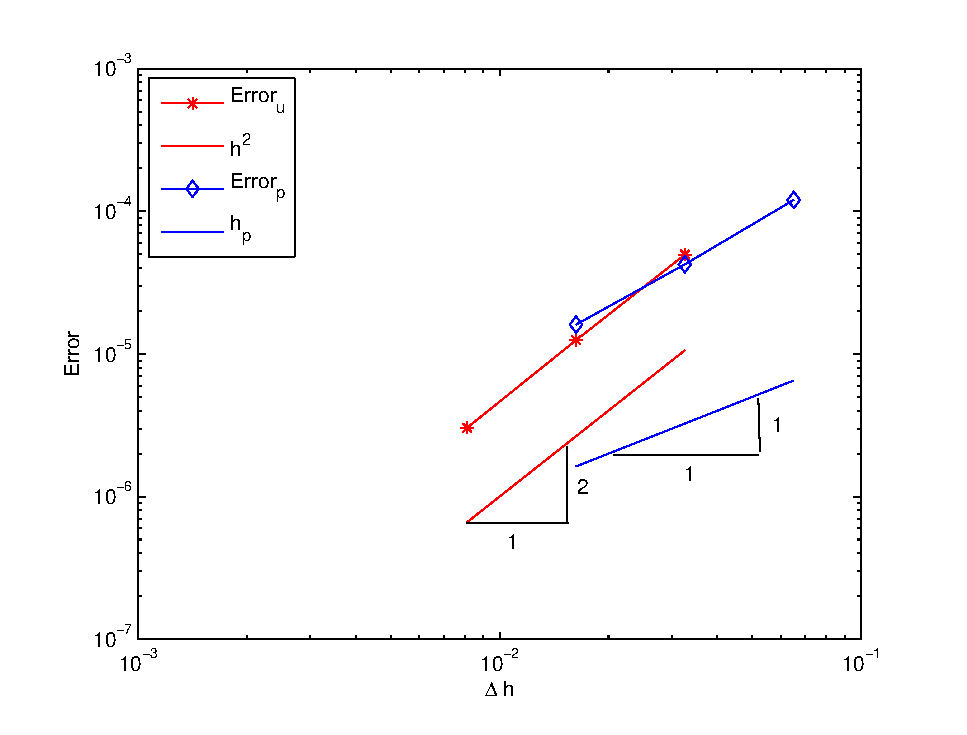
\includegraphics[width = 1.0\textwidth, angle =
           0]{picture/accuracy_flow/convergence_order.eps}
           \caption{Accuracy test:  The convergence order of $Error_u$ and $Error_p$
             with mesh refinement.}
           \label{fig::convergence_order}
       \end{figure}
       \begin{figure}
          \centering
          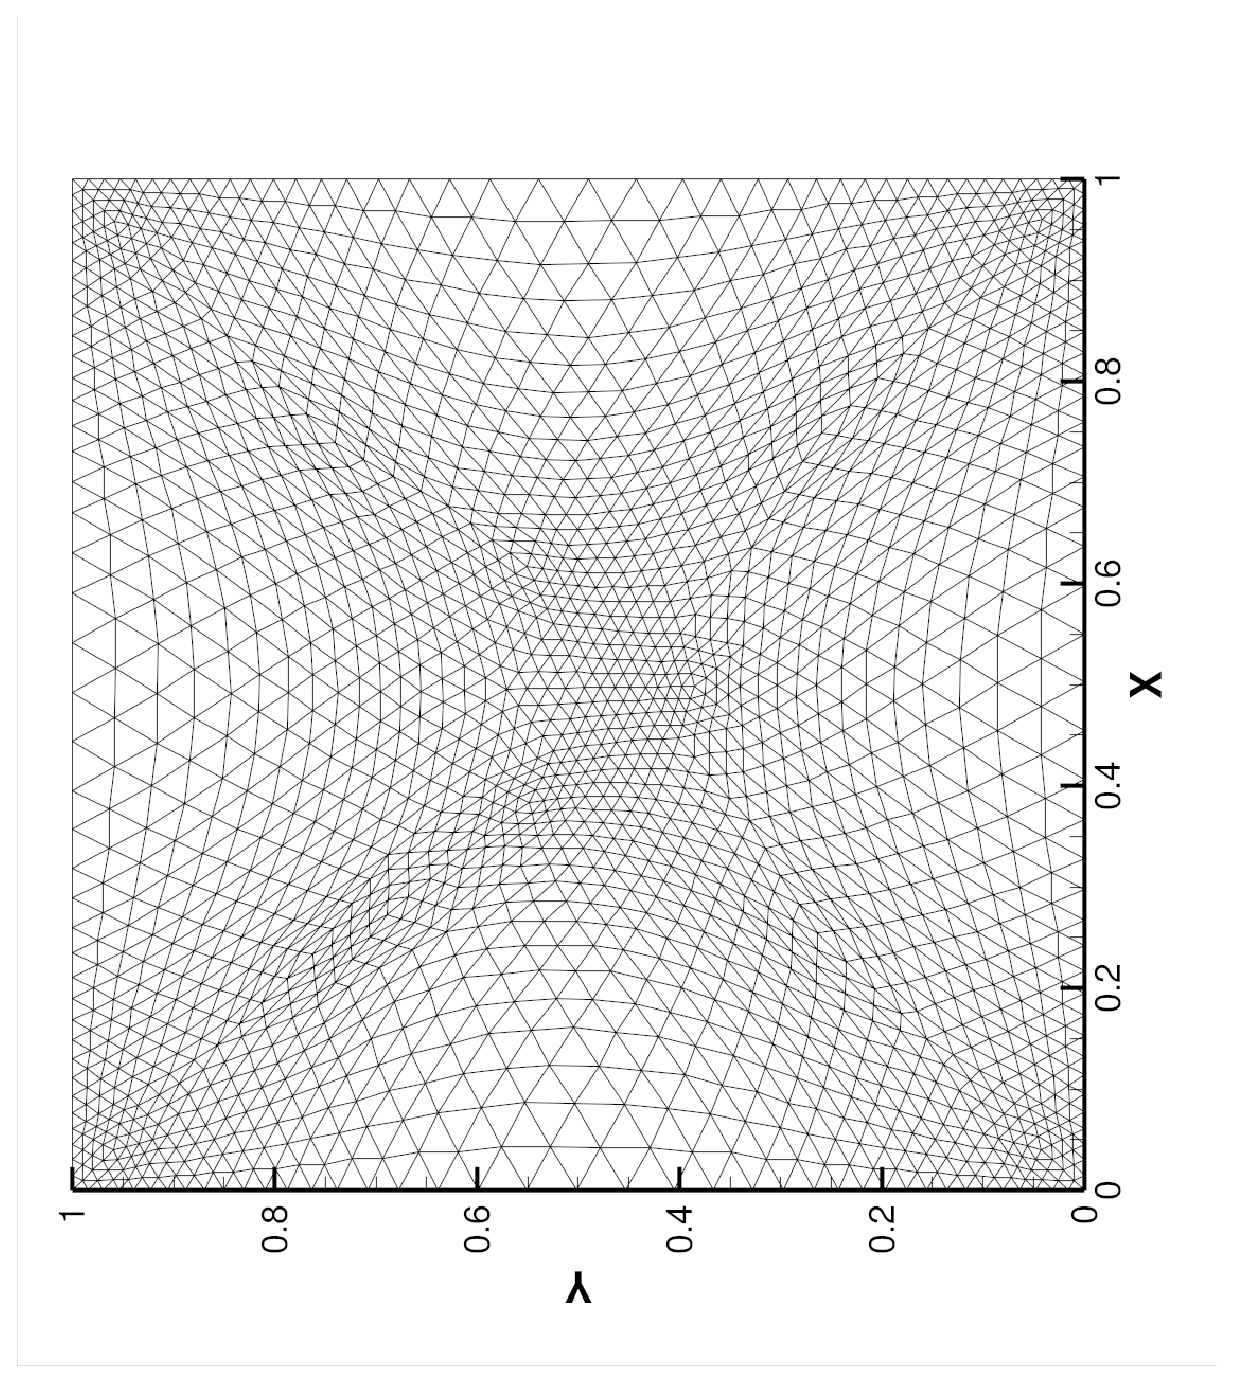
\includegraphics[width = 0.43\textwidth, angle = -90]{picture/accuracy_flow/accuray_mesh20.eps}
          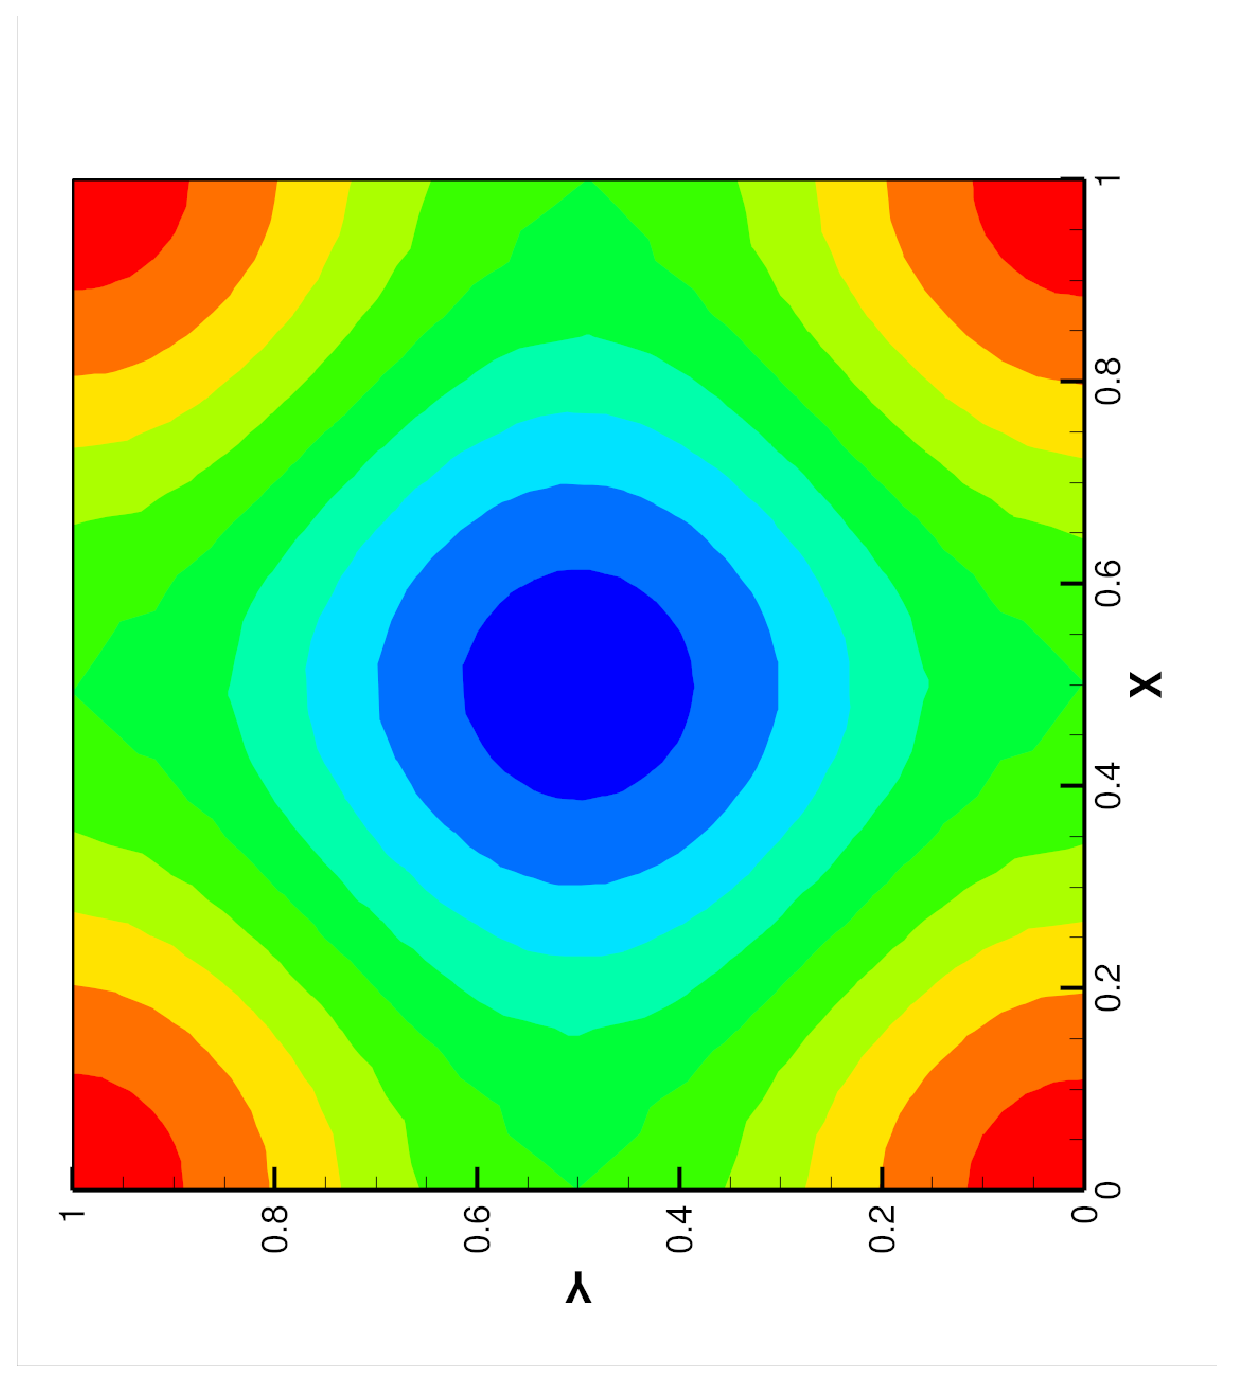
\includegraphics[width = 0.43\textwidth, angle = -90]{picture/accuracy_flow/pressure_mesh20.eps}
          \caption{\small Accuracy test: Moving mesh (left), pressure
            contour (right).}
        \label{fig::accuracy_mesh}
       \end{figure}
       
       % \begin{table}[!htbp]
       %   \centering
       %   \begin{tabular}{ccccccc}
       %     \toprule
       %      &\multicolumn{4}{c}{Accuracy of velocity }& \multicolumn{2}{c}{Accuracy of pressure} \\ \midrule
       %      velocity mesh   & $||\mathbf{u} - \mathbf{u}_h||_{L_2}$ &  order &
       %      $||\mathbf{u} - \mathbf{u}_h||_{H_1}$ & order & $||p - p_h||_{L_0}$  & order \\ \midrule
       %     $20 \times 20$   &  1.12e-1    &  & 3.19e1&     &   7.94e-1  &   
       %     \\ \midrule
       %     $40 \times 40$   &  2.82e-2   &  1.99  & 1.56e1 & 1.03 & 2.06e-1   &  1.95  
       %     \\ \midrule       
       %     $80 \times 80$   &  7.30e-3    &   1.95 & 8.02e-1 & 0.96& 5.74e-2   &  1.84
       %     \\ \bottomrule 
       %   \end{tabular}
       %   \caption{Accuracy test: accuracy check for the moving mesh
       %     solutions.}
       %   \label{tab::colliding_error}
       % \end{table}


       % \begin{equation}
       %   u_x = 20 xy^3, \quad u_y = 5x^4 - 5y^4, \quad p = 60x^2y -
       %   20y^3 + \mbox{constant}.
       % \label{eq::colliding_solution}
       % \end{equation}
       % Computational domain is $\Omega = [-1, 1]\times[-1, 1]$ and the velocity
       % in \eqref{eq::colliding_solution} is interpolated on all
       % boundary of $\Omega$.
       
       % We use this example to check the accuracy of our moving mesh
       % method. According to \cite{bercovier1979error}, the convergence
       % rate of velocity is second-order and pressure is first
       % order in the uniform mesh computation. Moving mesh algorithm is
       % applied to this example. We choose gradient-based monitor
       % \eqref{eq::monitor_gradient}, where user-defined parameters
       % $\alpha = 0.1, \beta = 1.0$. The $L_2$ error and $H_1$-semi error for the numerical
       % velocity, the $L_0$ error for the numerical pressure with
       % $\nu = 1.0$ are listed in Table \ref{tab::colliding_error}. It is discoverd that
       % velocity has a second-order accuracy and pressure has at least
       % first-order. Moving mesh and velocity streamline are shown in
       % Figure \ref{fig::colliding_mesh_streamline}.

       % \begin{figure}[!htbp]
       %   \begin{center}
       %       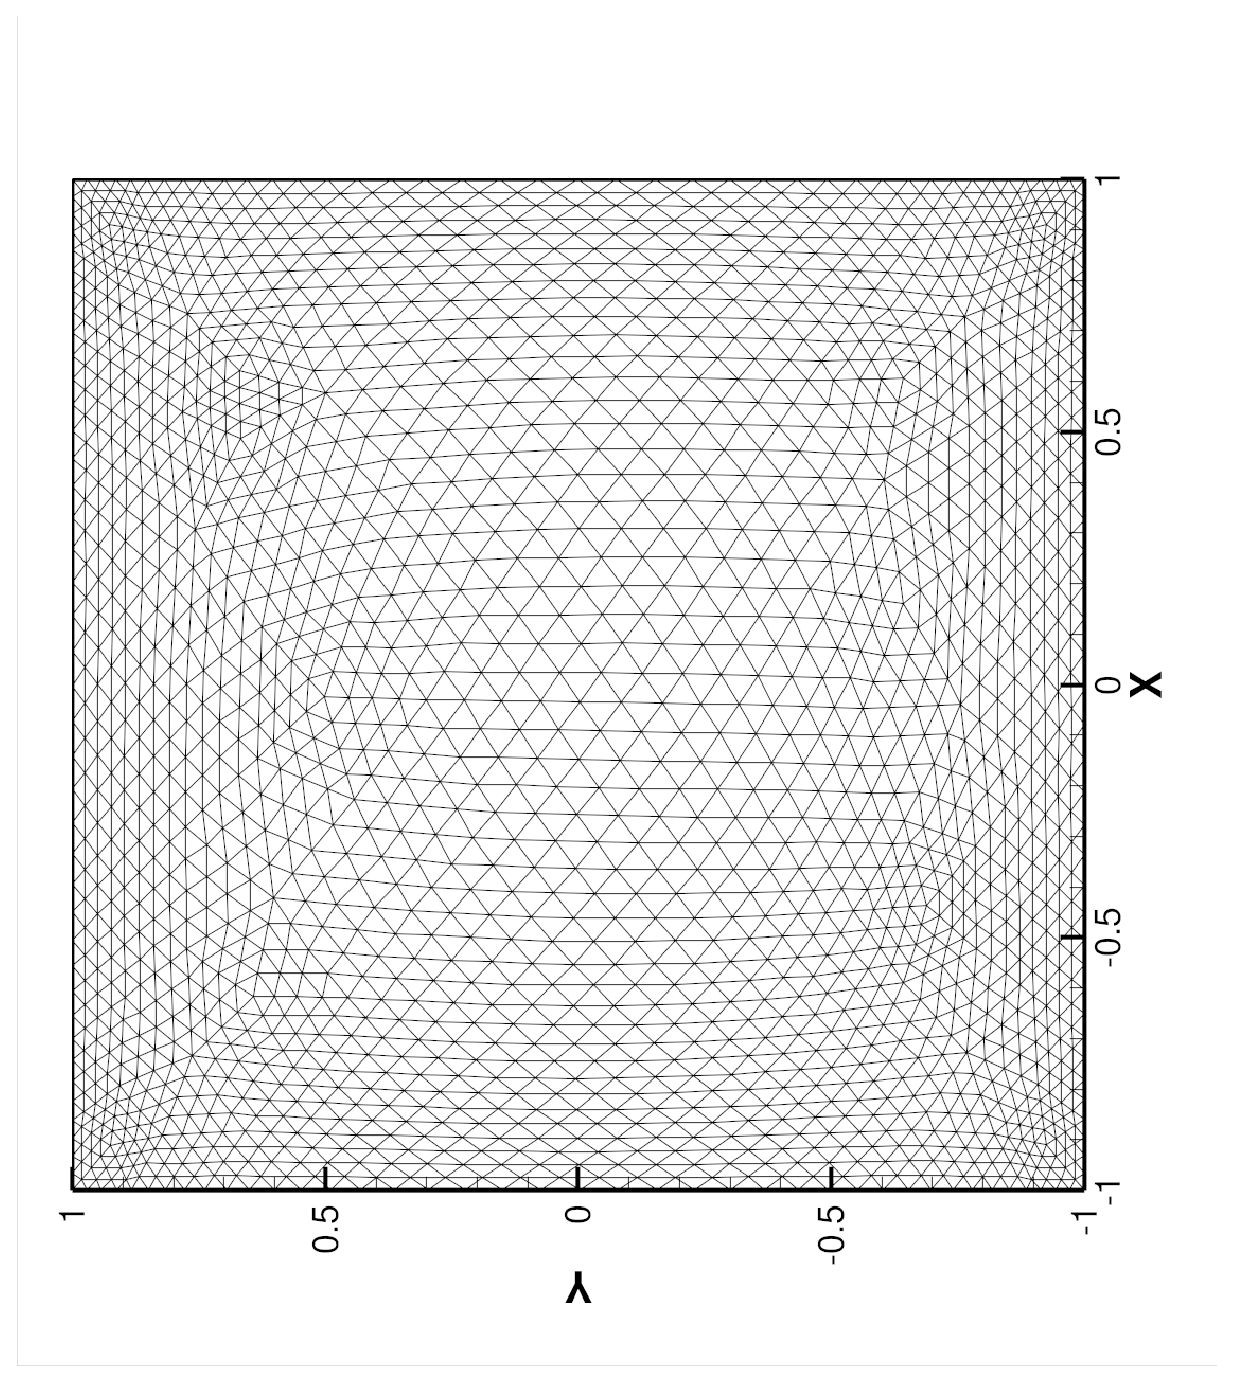
\includegraphics[width = 0.43\textwidth, angle = -90]{picture/colliding_flow_data/mesh20_01.eps}
       %       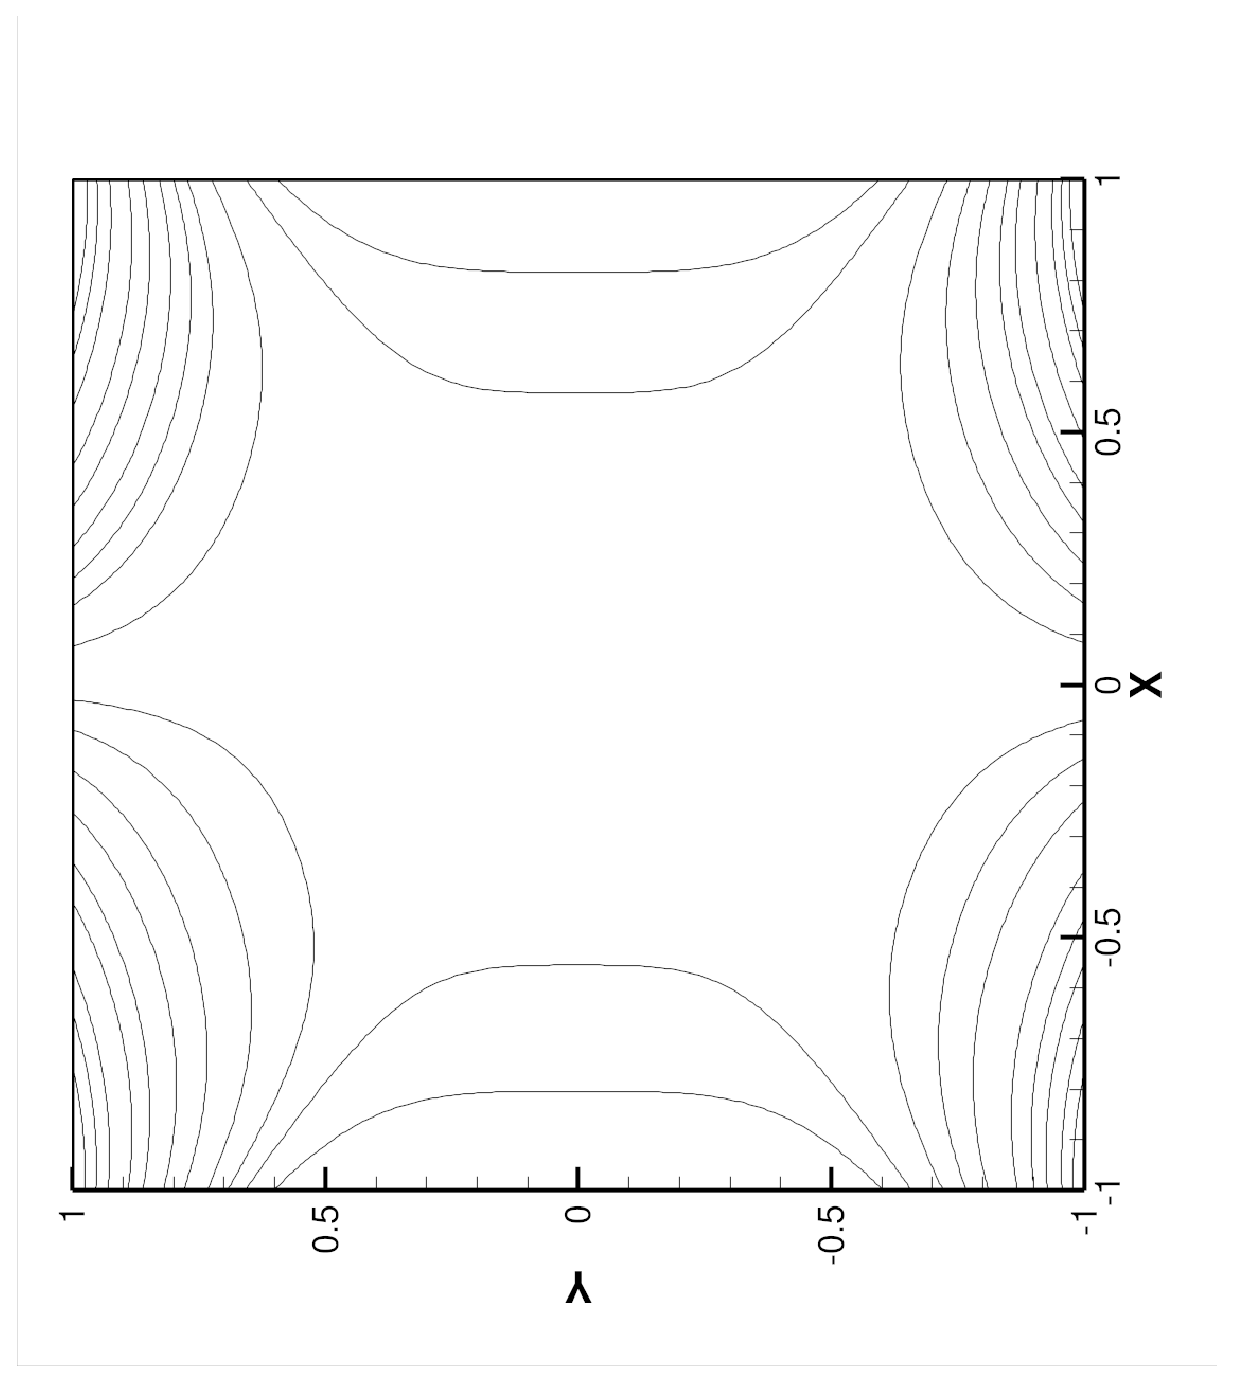
\includegraphics[width = 0.43\textwidth, angle = -90]{picture/colliding_flow_data/streamline20_01.eps}
       %  \end{center}
       %  \caption{\small Accuracy test: mesh (lest), streamline(right).}
       %  \label{fig::colliding_mesh_streamline}
       % \end{figure}
       
       % \begin{table}[!htbp]
       %   \centering
       %   \begin{tabular}{ccccccc}
       %     \toprule
       %      &\multicolumn{4}{c}{Accuracy of velocity }& \multicolumn{2}{c}{Accuracy of pressure} \\ \midrule
       %      velocity mesh   & $||\mathbf{u} - \mathbf{u}_h||_{L_2}$ &  order &
       %      $||\mathbf{u} - \mathbf{u}_h||_{H_1}$ & order & $||p - p_h||_{L_0}$  & order \\ \midrule
       %     $20 \times 20$   &  1.12e-1    &  & 3.19e1&     &   7.94e-1  &   
       %     \\ \midrule
       %     $40 \times 40$   &  2.82e-2   &  1.99  & 1.56e1 & 1.03 & 2.06e-1   &  1.95  
       %     \\ \midrule       
       %     $80 \times 80$   &  7.30e-3    &   1.95 & 8.02e-1 & 0.96& 5.74e-2   &  1.84
       %     \\ \bottomrule 
       %   \end{tabular}
       %   \caption{Accuracy test: accuracy check for the moving mesh
       %     solutions.}
       %   \label{tab::colliding_error}
       % \end{table}
       
       
     % \subsection{Jetting flow into a static field}
     %   This example models a thin flow jetting into a channel with
     %   static flow field.  
     %   Our computional domain is $\Omega = [0, 12] \times [-3, 3]$ and
     %   viscosity is $\nu = 0.0005$.
     %   Natural outflow boundary condition is imposed on $x = 12$,
     %   while inflow boundary condition $u_x = 1 - 100 y^2, u_y = 0$ on
     %   $x = 0, y \in [-0.1, 0.1]$. No-slip boundary condition is
     %   setted on other boundary of $\Omega$. 
       
     %   We select (\ref{eq::monitor_vorticity}) as monitor in our
     %   moving strategy. Parameters $\alpha = 2.0, \beta = 2.0$ perform
     %   well. As we known, when a thin flow jets into static
     %   field, two symmetric vortexes appears along the jetting flow.
     %   For improving the computional precision, it requires more grids
     %   around the flow. From Figure \ref{fig::jetting_flow_mesht12s}, mesh 
     %   is concentrated around the vorticity contour with large
     %   velocity gradient. As time evolving, fluid instability will apper
     %   Figure \ref{fig::jetting_flow_mesht27s} shown which is
     %   consistent with phisical phenomena.

     %   \begin{figure}[!htbp]
     %     \begin{center}
     %         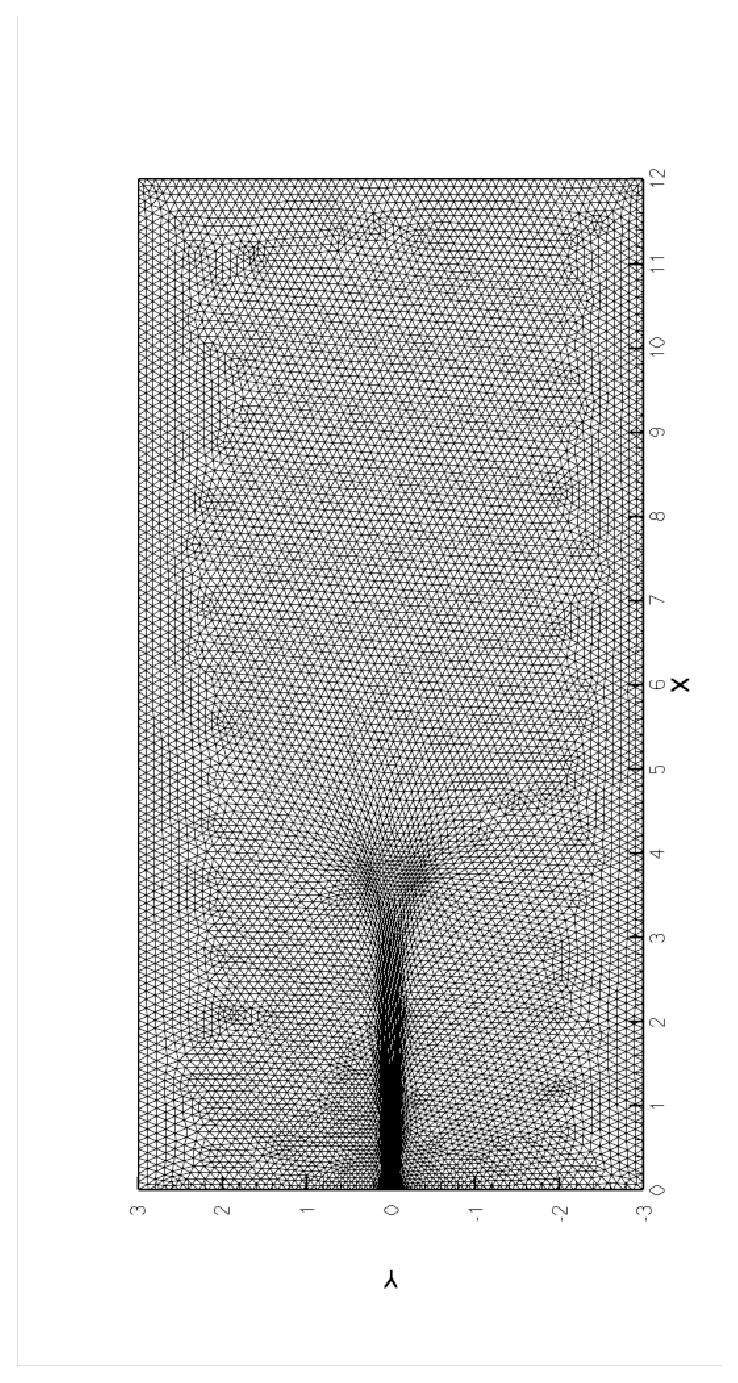
\includegraphics[width = 0.53\textwidth, angle = -90]{picture/jet_flow_data/mesh_t12s.eps}
     %         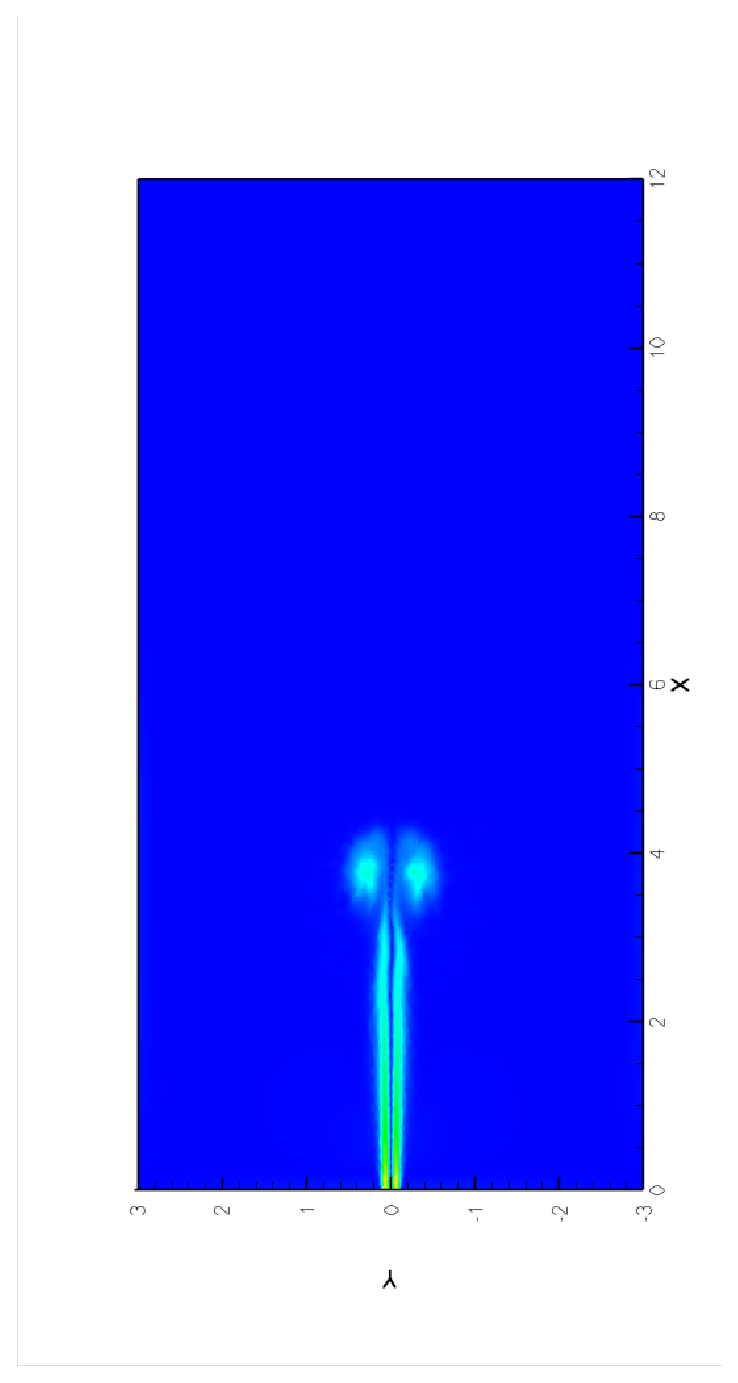
\includegraphics[width = 0.53\textwidth, angle = -90]{picture/jet_flow_data/contour_t12s.eps}
     %    \end{center}
     %    \caption{\small Jetting flow: top: mesh, bottom: vorticity contour at t = 12.}
     %    \label{fig::jetting_flow_mesht12s}
     %   \end{figure}

     %   \begin{figure}[!htbp]
     %     \begin{center}
     %         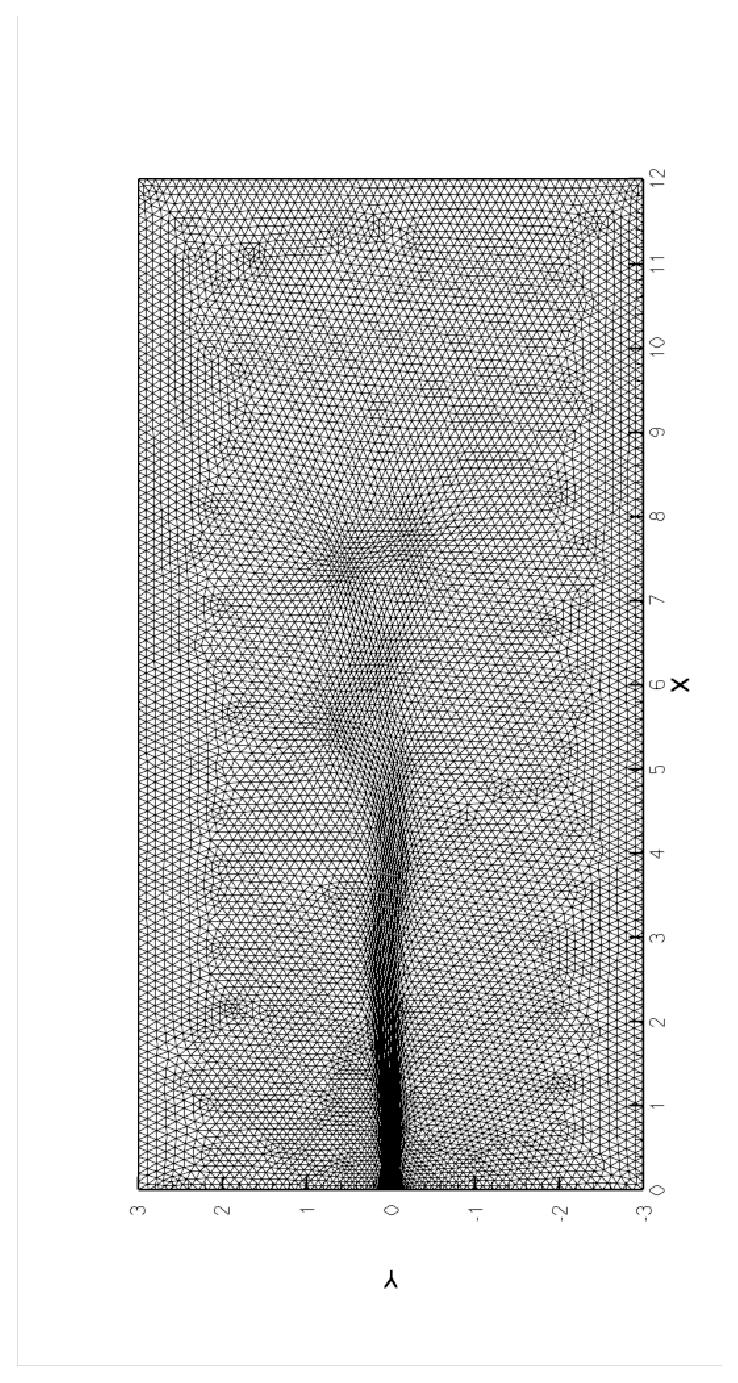
\includegraphics[width = 0.53\textwidth, angle = -90]{picture/jet_flow_data/mesh_t27s.eps}
     %         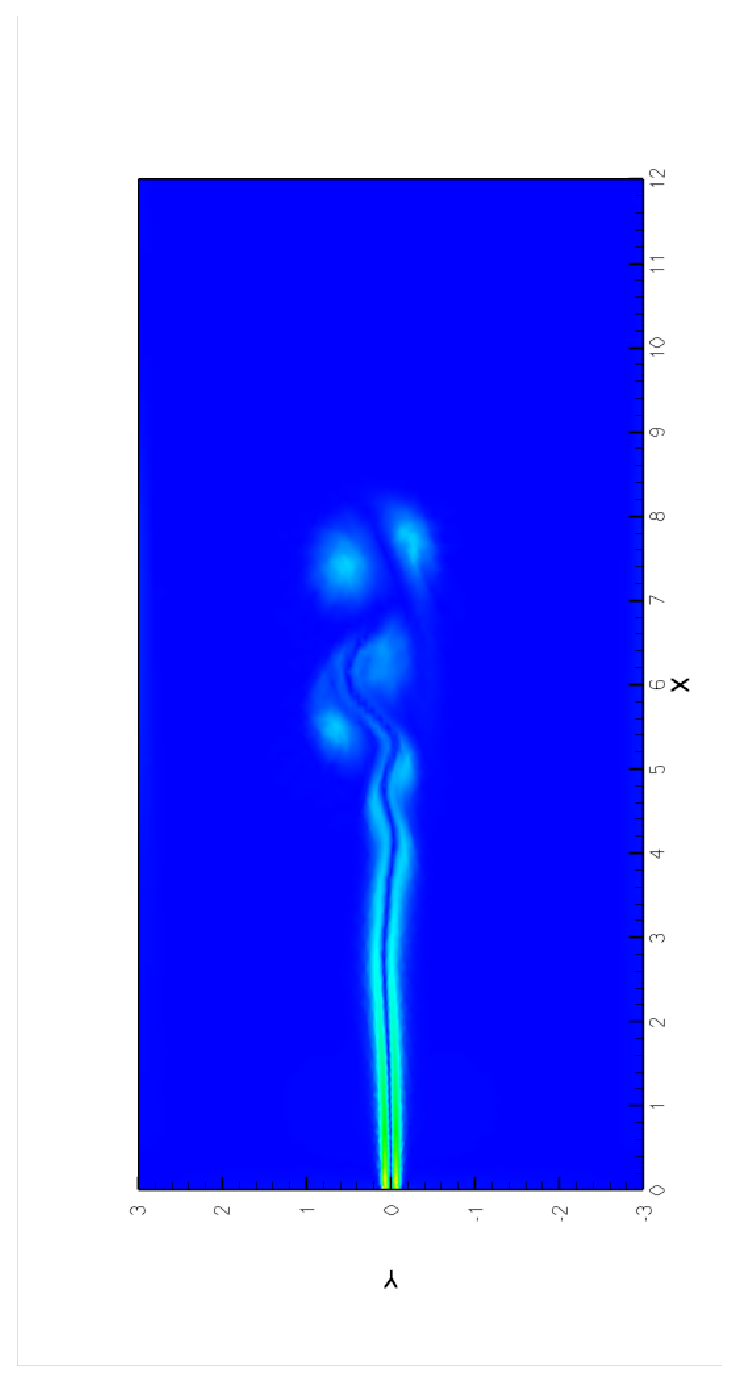
\includegraphics[width = 0.53\textwidth, angle = -90]{picture/jet_flow_data/contour_t27s.eps}
     %    \end{center}
     %    \caption{\small Jetting flow: top: mesh, bottom: vorticity contour at t = 27.}
     %    \label{fig::jetting_flow_mesht27s}
     %   \end{figure}
       

   \subsection{Navier-Stokes flow over a step}

      We consider the test problem in \cite{zheng2010adaptive} that the
      Navier-Stokes flow over a step with $\text{Re} = 1000$. The
      domain is $\Omega = (0, 4) \times (0, 1)/(1.2, 1.6) \times (0,
      0.4)$, and on the upper and bottom boudaries, Dirichlet
      condition $\mathbf{u} = (0, 0)^T$ is imposed. Outflow boundary is
      enforced natural boundary condition meanwhile at the inflow
      boundary $\mathbf{u} = (4 y (1 - y), 0)$.

      Vorticity-based monitor (\ref{eq::monitor_vorticity}) is
      selected as monitor with $\alpha = 0.4, \beta =
      2.0$. As we known, singularities arise due to the concave corner in this
      problem. The development of
      moving mesh and vorticity contour as time evolving are show in Figure
      \ref{fig::step_flow_3s} and \ref{fig::step_flow_20s}. % show moving mesh and contour of
      % vorticity at $t = 0.5, t = 1 \text{, and } t = 2$.
      It can be observed that mesh clusters near the top concave edge
      and moving mesh is consistent with the structure of vorticity.

      In Figure \ref{fig::step_flow_pressure_contour_20s}, the
      comparation of pressure contour with uniform mesh and moving
      mesh at $t = 20$ are shown. In the uniform case, numerical
      dissipation is introduced. While better representation of
      pressure contour with less dissipation is obtained in the moving case.    
       

      % \begin{figure}[!htbp]
      %   \centering
      %   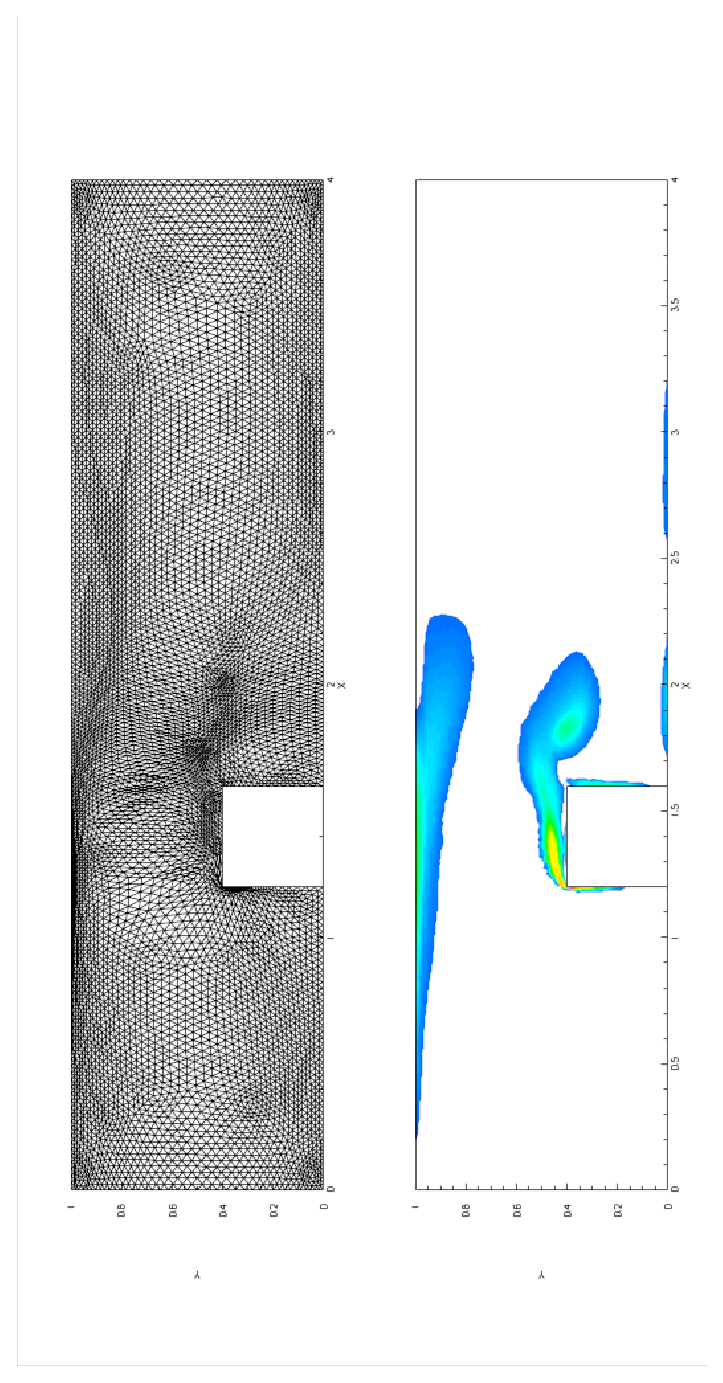
\includegraphics[width = 0.55\textwidth, angle = -90]{picture/step_flow_data/mesh_t_05.eps}
      %   \caption{\small Top: moving mesh; bottom: contour of vorticity
      %     at t = 0.5.}
      %   \label{fig::step_flow_05s}
      % \end{figure}

      % \begin{figure}[!htbp]
      %   \centering
      %   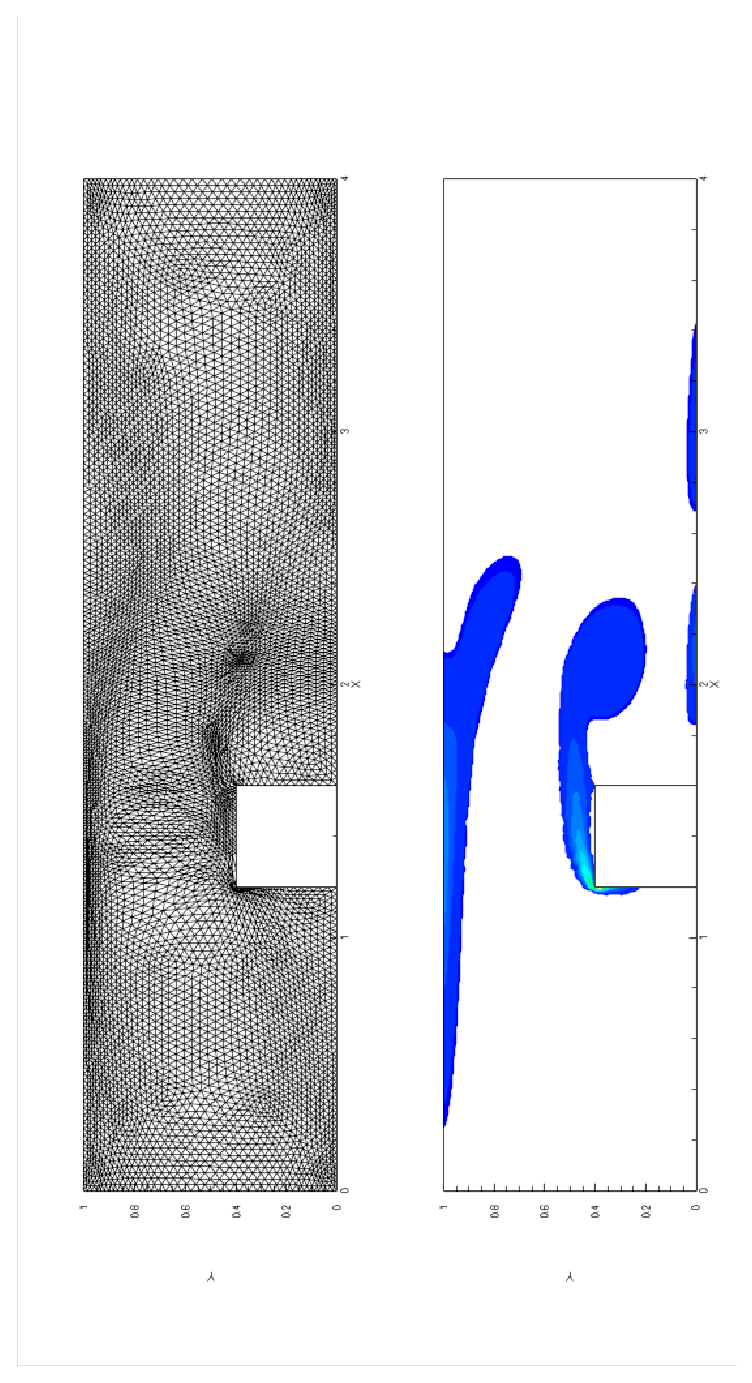
\includegraphics[width = 0.55\textwidth, angle = -90]{picture/step_flow_data/mesh_t_1s.eps}
      %   \caption{\small Top: moving mesh; bottom: contour of vorticity
      %     at t = 1.}
      %   \label{fig::step_flow_1s}
      % \end{figure}

      % \begin{figure}[!htbp]
      %   \centering
      %   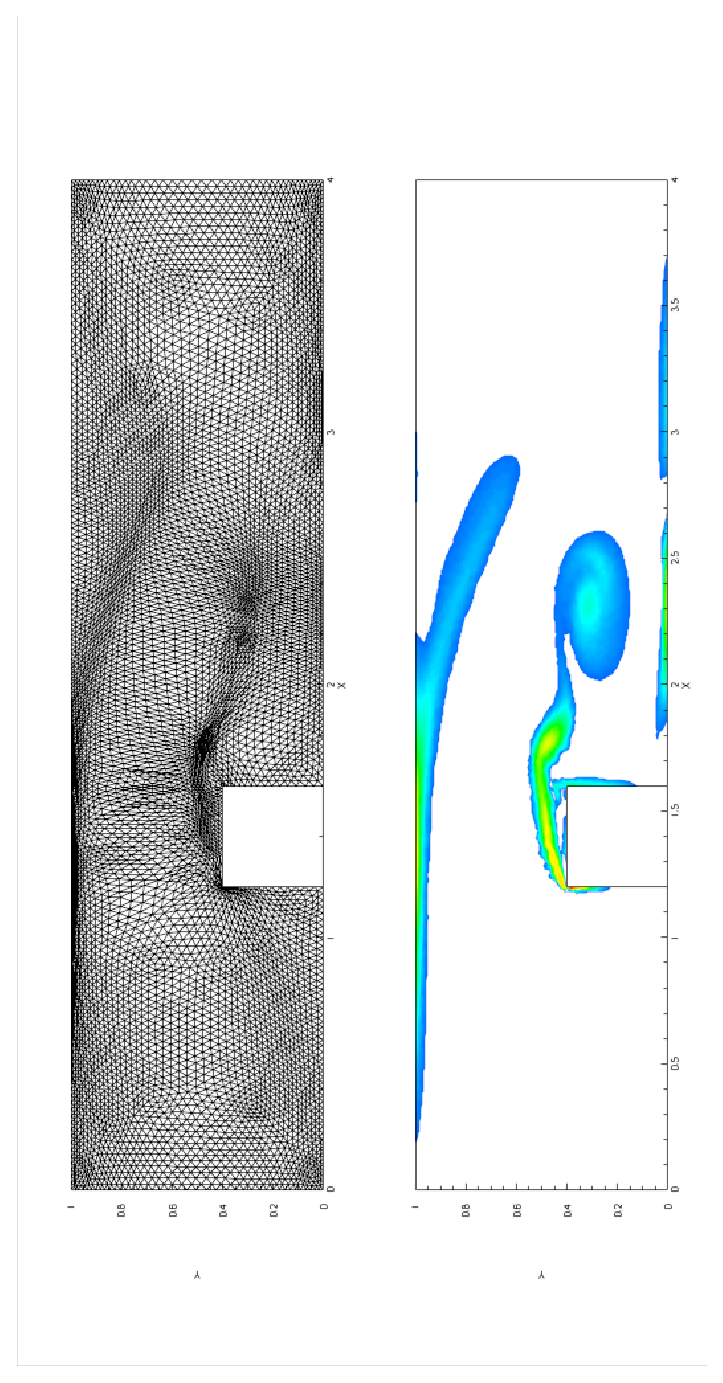
\includegraphics[width = 0.55\textwidth, angle = -90]{picture/step_flow_data/mesh_t_1_5s.eps}
      %   \caption{\small Top: moving mesh; bottom: contour of vorticity
      %     at t = 1.5.}
      %   \label{fig::step_flow_1_5s}
      % \end{figure}

      \begin{figure}[!htbp]
        \centering
        \subfloat[t = 1] {
          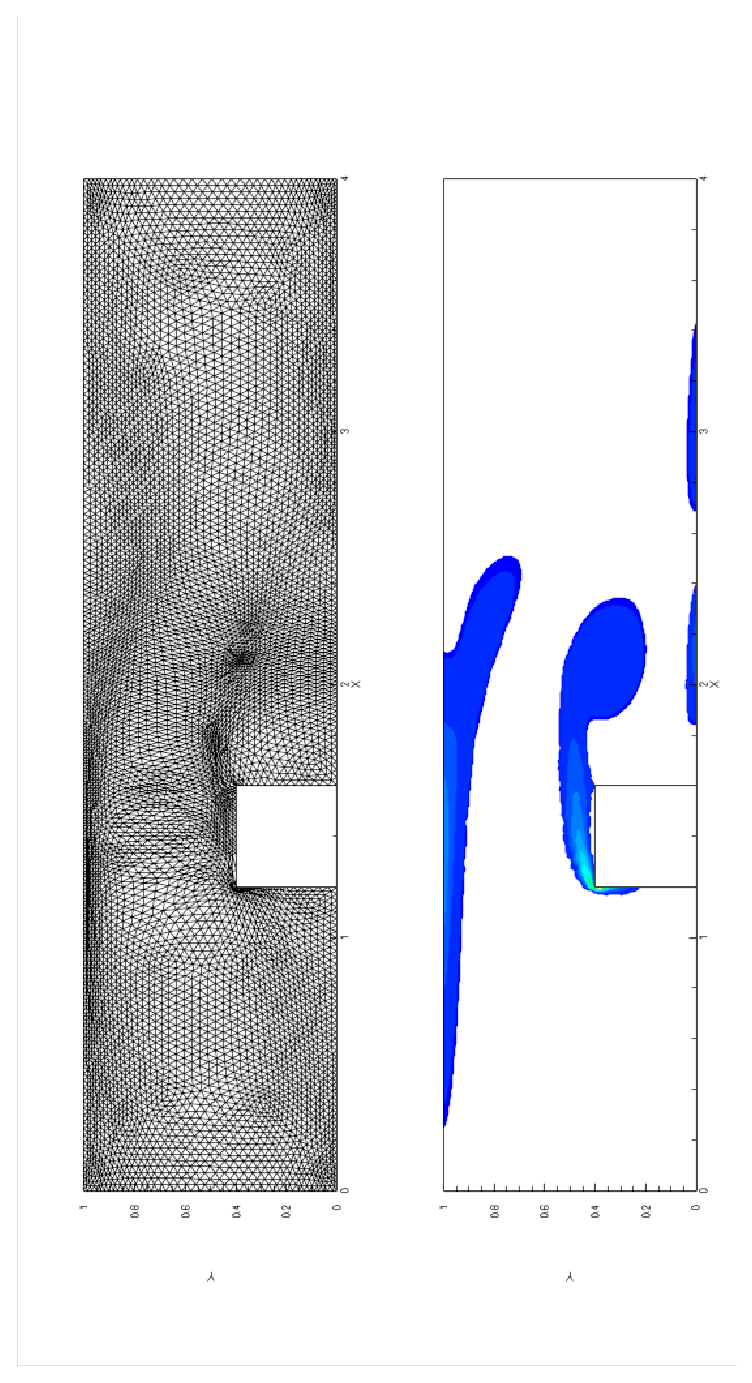
\includegraphics[width = 0.25\textwidth, angle = -90]{picture/step_flow_data/mesh_t_1s.eps}
          }
        \subfloat[t = 3] {
          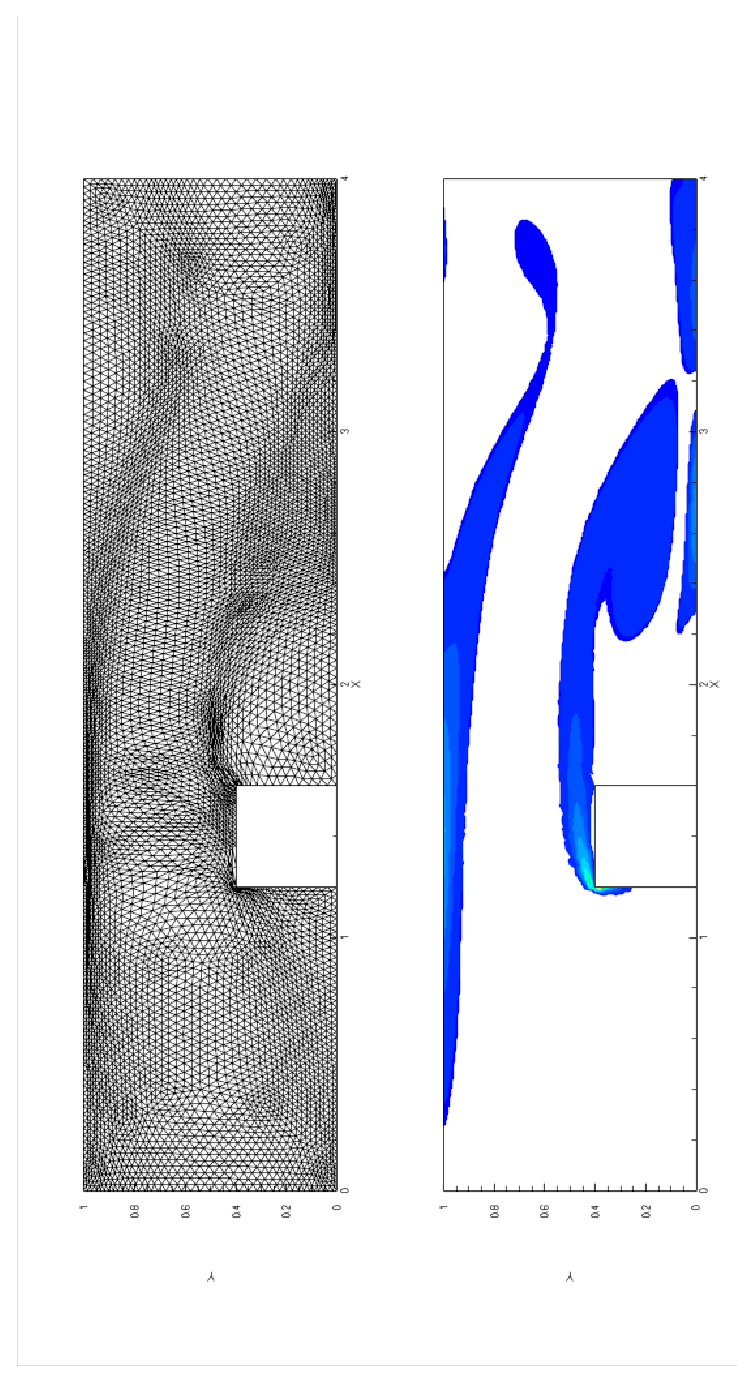
\includegraphics[width = 0.25\textwidth, angle = -90]{picture/step_flow_data/mesh_t_3s.eps}
        }
        \caption{\small Top: moving mesh; bottom: contour of vorticity.}
        \label{fig::step_flow_3s}
      \end{figure}

      \begin{figure}[!htbp]
        \centering
        \subfloat[t = 7] {
          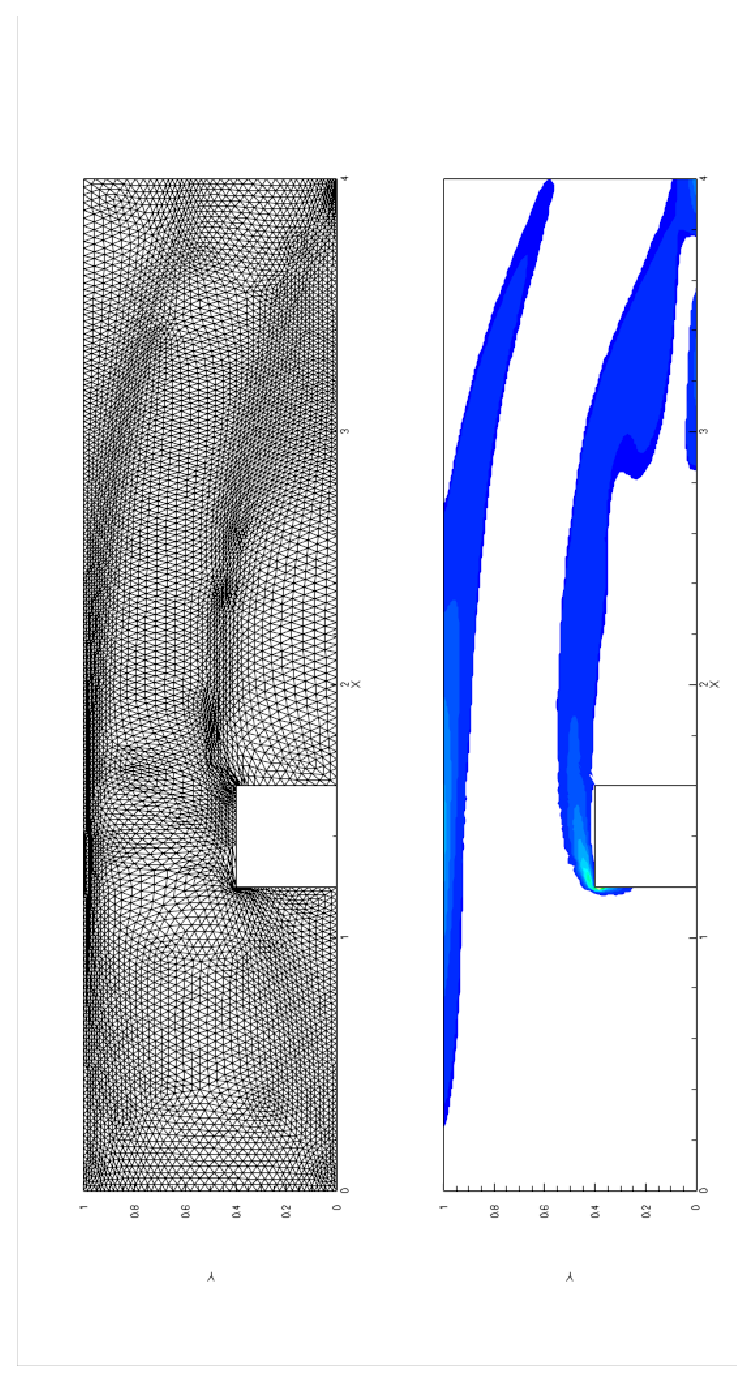
\includegraphics[width = 0.25\textwidth, angle = -90]{picture/step_flow_data/mesh_t_7s.eps}
          }
        \subfloat[t = 20] {
          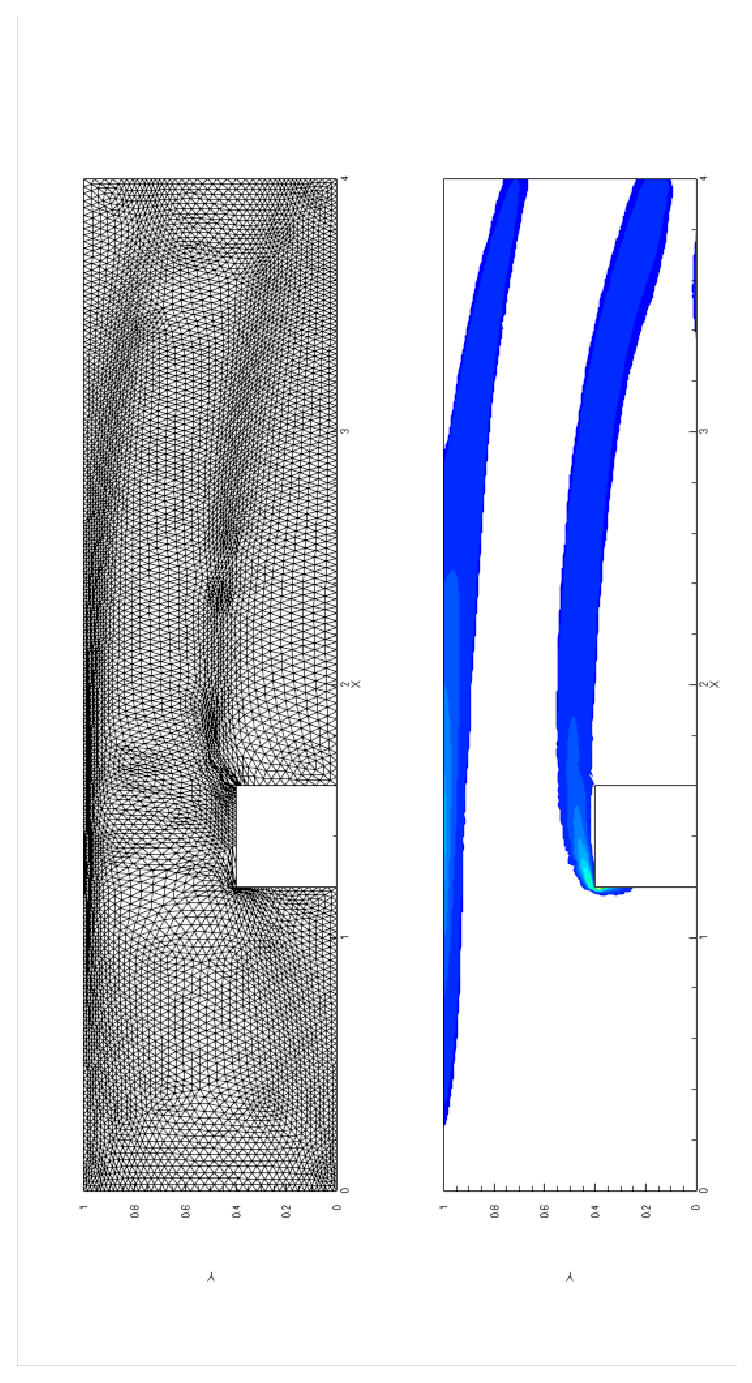
\includegraphics[width = 0.25\textwidth, angle = -90]{picture/step_flow_data/mesh_t_20s.eps}
        }
        \caption{\small Top: moving mesh; bottom: contour of vorticity.}
        \label{fig::step_flow_20s}
      \end{figure}

      \begin{figure}[!htbp]
        \centering
        \includegraphics[width = 0.55\textwidth, angle = -90]{picture/step_flow_data/pressure_contour.eps}
        \caption{\small Pressure contour: moving mesh (top); uniform
          mesh (bottom) at t = 20.}
        \label{fig::step_flow_pressure_contour_20s}
      \end{figure}

   \subsection{Flow over cylinder}
   
      This example models the development of flow over an cylinder
      along a retangular channel. In \cite{cao1999anr}, the authors
      apply moving finite element method to this problem. The center
      of cylinder is $(0, 0)$ and radius is $r = 0.3$. Let Reynolds 
      number $Re = 300$ and domain $\Omega = [-1, 5] \times [-1, 1]$. 
      Poiseuille flow $u = 1 - y^2, v = 0$ is imposed on inflow
      boundary $x = -1$. $u = v = 0$ is imposed on the top and bottom
      of the channel. Outflow boundary $x = 5$ is natrual
      condition. 

      If we concern the fine flow structure, it is required
      high resolution for small scale structure. For detecting the
      vorticity, (\ref{eq::monitor_vorticity}) is a good choice as the
      monitor in our moving strategy. The parameters $\alpha$ and
      $\beta$ are $1.0$, $2.0$. 

      In Figure \ref{fig::cylinder_initial_mesh}, initial moving mesh
      is shown clustering near the circular cylinder where need high
      resolution. The evolution of
      moving mesh and vorticity contour are illustrated in Figure
      \ref{fig::cylinder_mesh_t24_5s}. It can be discoverd that our
      moving mesh can efficiently capture the vorticity structure and
      our mesh is more concentrated than \cite{cao1999anr}. Velocity
      streamline is shown in Figure
      \ref{fig::cylinder_streamline_t24_5s}.

      
      % When we change the value of viscosity $\nu = 0.001$, the
      % structure of moving mesh and vorticity contour are not so
      % obvious as viscosity $\nu = 0.003$, as shown in 
      % Figure \ref{fig::cylinder_mesh_t23s}. 
      
      \begin{figure}[!htbp]
        \centering
        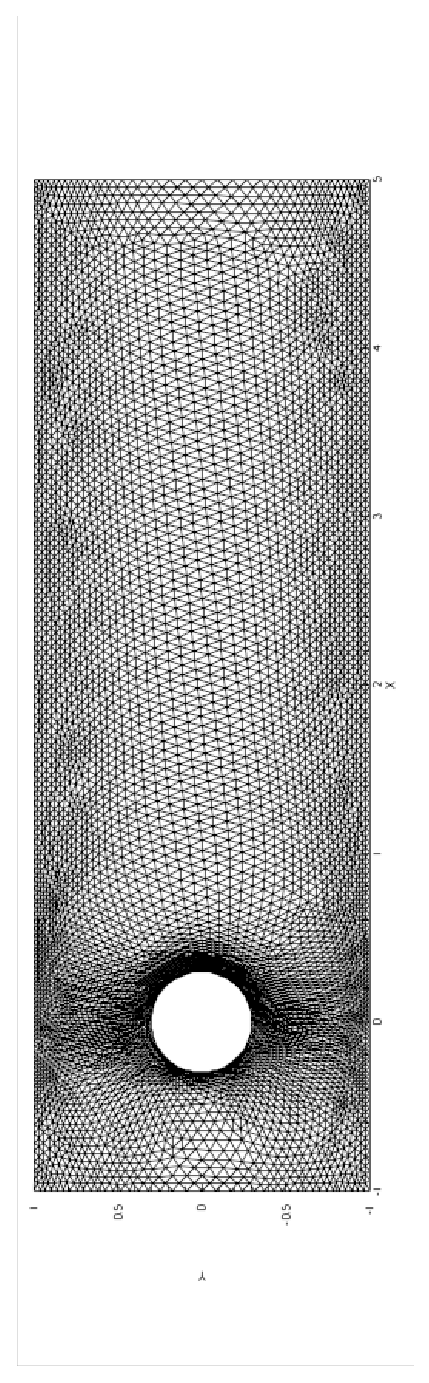
\includegraphics[width = 0.3\textwidth, angle = -90]{picture/obstacle_flow_data/initial_mesh.eps}
        \caption{\small Initial moving mesh, $Re = 300$.}
        \label{fig::cylinder_initial_mesh}
      \end{figure}

      \begin{figure}[!htbp]
       \begin{center}
         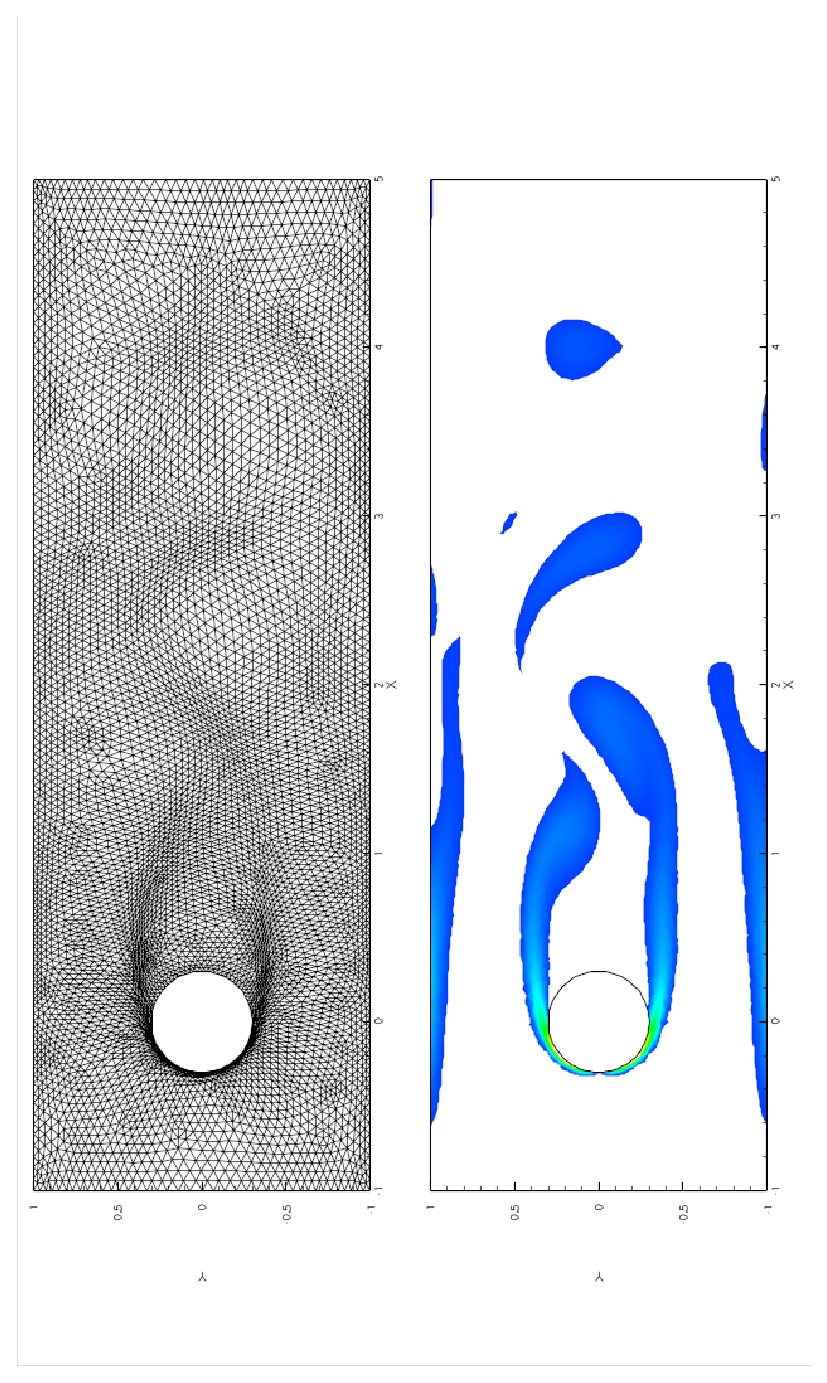
\includegraphics[width = 0.6\textwidth, angle = -90]{picture/obstacle_flow_data/mesh_t_24_5s.eps}
       \end{center}  
       \caption{\small Top: moving mesh; bottom: vorticity contour at
         $t = 24.5$, $Re = 300$.}
       \label{fig::cylinder_mesh_t24_5s}
     \end{figure}

      \begin{figure}[!htbp]
       \begin{center}
         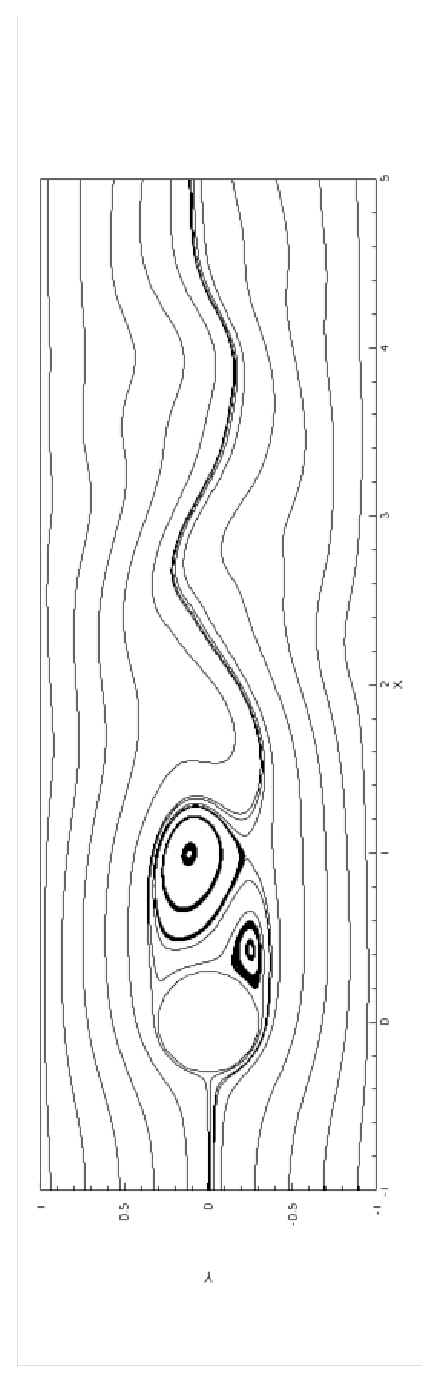
\includegraphics[width = 0.3\textwidth, angle = -90]{picture/obstacle_flow_data/streamline_t_24_5s.eps}
       \end{center}  
       \caption{\small Top: vorticity streamline at $t = 24.5$, $Re = 300$.}
       \label{fig::cylinder_streamline_t24_5s}
     \end{figure}

     % \begin{figure}[!htbp]
     %   \centering
     %   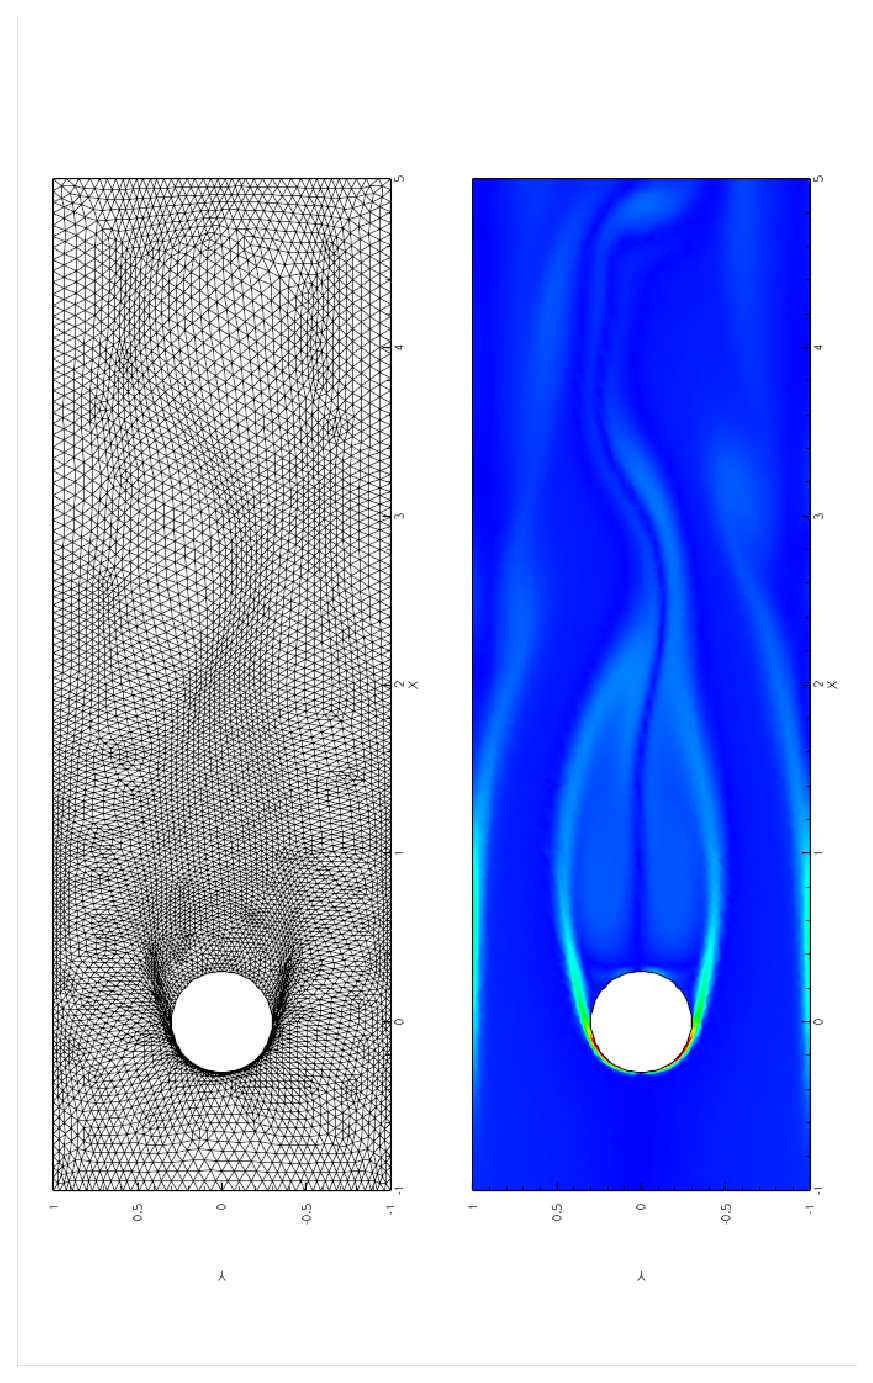
\includegraphics[width = 0.6\textwidth, angle = -90]{picture/obstacle_flow_data/mesh_t_23s.eps}
     %   \caption{\small Top: moving mesh; bottom: vorticity contour at
     %     $t = 23$, viscosity $\nu = 0.001$.}
     %   \label{fig::cylinder_mesh_t23s}
     % \end{figure}

%%% Remarks %%%%%%%%
\section{Remarks}
   \label{sec8} In this paper, unsteady Navier-Stokes equations have
   been numerically solved using moving mesh method on $4P_1-P_1$
   element. Hierarchy geometry tree is used to  store the
   mesh structure of $4P_1-P_1$ element. This pair natrually satisfies 
   LBB condition and it's reference element has only $P_1$ element.
   
   Hierarchy geometry tree structure make convienence for multigrid
   preconditioning. However, the preconditioning strategy isn't
   implemented for Navier-Stokes system in this work. But it will
   appear in future work. Meanwhile, this tree structure is originally
   used for h-adaptive mesh. So the combining moving mesh with
   h-adaptive mesh by making use of this tree structure will be also
   considered.
 
    
   % $4P_1-P_1$ element pair natrually satisfies the LBB confiditon and is
   % linear-order element. In practical engeneering computation,
   % linear-order element is more popular than high order because of its
   % simplicity and complexity of problems. For capturing the fine flow
   % structure, we apply moving mesh method to this pair using vorticity
   % as monitor. The moving mesh is consistent with the structure of
   % vorticity. Boundary conditions in our testing problem are all
   % non-periodic, so it has more extensive application.
   
   % Our mesh structure is based on the hierarchy geometry tree
   % structure, multi-mesh adaptive method will be applied to $4P_1-P_1$
   % pair. Also moving mesh method for incompressible flow will be
   % extended to three-dimention in future work. 

%%%% Acknowledgments %%%%%%%%
\section*{Acknowledgments}
The authors' work was supported in part by the National Basic Research
Program of China(2011CB309704) and the National Natrual Science
Foundation of China(11271358 and 91230108).
   
%%%% Bibliography  %%%%%%%%%%
\bibliographystyle{unsrt}
%include mathpaper.bib文件.
\bibliography{mathpaper}
% ----------------------------------------------------------------------------------------


 \end{document}
